\documentclass[sigconf]{acmart}
% 
% LaTeX template for visualizing the performance of
% optimization algorithms, that were run on the 
% bbob-mmixint test suite of COCO. Any number of 
% algorithms should work with this template.
%


\usepackage{booktabs} % For formal tables
\usepackage{graphicx}
\usepackage{rotating}
\definecolor{Gray}{gray}{0.6}
\usepackage{tabularx}
\usepackage{xspace}
\usepackage{float}
\usepackage{xstring} % for string operations
\usepackage{wasysym} % Table legend with symbols input from post-processing
\usepackage{MnSymbol} % Table legend with symbols input from post-processing
\usepackage{ifthen}
\newcommand{\includeperfprof}[1]{% include and annotate at the side
  \input{\bbobdatapath\algsfolder #1}%
  \includegraphics[height=0.24\textheight]{#1}%
  %\raisebox{.12\textheight}{
	%\parbox[b][.24\textheight]{.0868\textwidth}{\begin{scriptsize}
  %  \perfprofsidepanel % this is "\algaperfprof \vfill \algbperfprof \vfill" etc
  %\end{scriptsize}}
	%}
}





% Copyright
%\setcopyright{none}
%\setcopyright{acmcopyright}
%\setcopyright{acmlicensed}
\setcopyright{rightsretained}
%\setcopyright{usgov}
%\setcopyright{usgovmixed}
%\setcopyright{cagov}
%\setcopyright{cagovmixed}


% DOI
\acmDOI{10.1145/123_4}

% ISBN
\acmISBN{123-4567-24-567/18/07}

%Conference
\acmConference[GECCO '19]{the Genetic and Evolutionary Computation Conference 2019}{July 13--17, 2019}{Prague, Czech Republic}
\acmYear{2019}
\copyrightyear{2019}

\acmPrice{15.00}

%%%%%%%%%%%%%%%%%%%%%%%%%%%%%%%%%%%%%%%%%%%%%%%%%%%%%%%%%%%%%%%%%%%%%%%%%%%%%%%
%%%%%%%%% TO BE EDITED %%%%%%%%%%%%%%%%%%%%%%%%%%%%%%%%%%%%%%%%%%%%%%%%%%%%%%%%
%%%%%%%%%%%%%%%%%%%%%%%%%%%%%%%%%%%%%%%%%%%%%%%%%%%%%%%%%%%%%%%%%%%%%%%%%%%%%%%

% Algorithm names as they appear in the tables, uncomment and adapt if necessary
% \newcommand{\algAtables}{ALGO1}  % first argument in the post-processing
% \newcommand{\algBtables}{ALGO2}  % second argument in the post-processing
% \newcommand{\algCtables}{ALGO3}  % third argument in the post-processing
% \newcommand{\algDtables}{ALGO4}  % forth argument in the post-processing
% ...
% location of pictures files
\newcommand{\bbobdatapath}{ppdata/} % change default output folder of COCO if desired



%%%%%%%%%%%%%%%%%%%%%%%%%%%%%%%%%%%%%%%%%%%%%%%%%%%%%%%%%%%%%%%%%%%%%%%%%%%%%%%
% read in data and deal with the different number of algorithms:
\input{\bbobdatapath cocopp_commands.tex}

\ifthenelse{\equal{\numofalgs}{1}}{
   \graphicspath{{\bbobdatapath\algfolder}}}{
	 \graphicspath{{\bbobdatapath\algsfolder}}
}

\ifthenelse{\isundefined{\algorithmA}}{\newcommand{\algorithmA}{\algname}}{}
%\ifthenelse{\isundefined{\algorithmA}{\newcommand{\algorithmA}{\change{MY-ALGORITHM-NAME}}}{}  % better use the previous line?
%%



%%%%%%%%%%%%%%%%%%%%%%%%%%%%%%%%%%%%%%%%%%%%%%%%%%%%%%%%%%%%%%%%%%%%%%%%%%%%%%%
%%%%%%%%%%%%%%%%%%%%%%%%%%%%%%%%%%%%%%%%%%%%%%%%%%%%%%%%%%%%%%%%%%%%%%%%%%%%%%%
%%%%%%%%%%%%%%%%%%%%%%%%%%%%%%%%%%%%%%%%%%%%%%%%%%%%%%%%%%%%%%%%%%%%%%%%%%%%%%%

\newcommand{\DIM}{\ensuremath{\mathrm{DIM}}}
\newcommand{\ERT}{\ensuremath{\mathrm{ERT}}}
\newcommand{\FEvals}{\ensuremath{\mathrm{FEvals}}}
\newcommand{\nruns}{\ensuremath{\mathrm{Nruns}}}
\newcommand{\Dfb}{\ensuremath{\Delta f_{\mathrm{best}}}}
\newcommand{\Df}{\ensuremath{\Delta f}}
\newcommand{\DI}{\ensuremath{\Delta I_{\mathrm{HV}}^{\mathrm{COCO}}}}
\newcommand{\nbFEs}{\ensuremath{\mathrm{\#FEs}}}
\newcommand{\ftarget}{\ensuremath{f_\mathrm{t}}}
\newcommand{\Itarget}{\ensuremath{I_\mathrm{target}}}
\newcommand{\CrE}{\ensuremath{\mathrm{CrE}}}
\newcommand{\hvref}{\ensuremath{I_\mathrm{ref}}}
\newcommand{\fopt}{\hvref}
\newcommand{\change}[1]{{\color{red} #1}}
\newcommand{\TODO}[1]{{\color{orange} !!! #1 !!!}}
\newcommand{\bbobbiobj}{{\ttfamily bbob-biobj}\xspace}
\newcommand{\bbobnoisy}{{\ttfamily bbob-noisy}\xspace}
\newcommand{\bbobmixint}{{\ttfamily bbob-mixint}\xspace}
\newcommand{\rot}[2][2.5]{
  \hspace*{-3.5\baselineskip}%
  \begin{rotate}{90}\hspace{#1em}#2
  \end{rotate}}

%%%%%%%%%%%%%%%%%%%%%%   END OF PREAMBLE   %%%%%%%%%%%%%%%%%%%%%%%%%%%%%%%%%%%%

\begin{document}


\title{Black-Box Optimization Benchmarking Template for the Comparison of Algorithms on the \bbobmixint Testbed}
\renewcommand{\shorttitle}{Template to Compare Algorithms on the \bbobmixint Testbed}
\titlenote{Submission deadline: April 3rd.}
%Camera-ready paper due April 24th.}}
\subtitle{Draft version}



\author{Firstname Lastname}
%\authornote{tba if needed}
%\orcid{1234-5678-9012}
%\affiliation{%
%  \institution{Institute for Clarity in Documentation}
%  \streetaddress{P.O. Box 1212}
%  \city{Dublin} 
%  \state{Ohio} 
%  \postcode{43017-6221}
%}
%\email{trovato@corporation.com}
%
%\author{G.K.M. Tobin}
%\authornote{The secretary disavows any knowledge of this author's actions.}
%\affiliation{%
%  \institution{Institute for Clarity in Documentation}
%  \streetaddress{P.O. Box 1212}
%  \city{Dublin} 
%  \state{Ohio} 
%  \postcode{43017-6221}
%}
%\email{webmaster@marysville-ohio.com}
%
%\author{Lars Th{\o}rv{\"a}ld}
%\authornote{This author is the
%  one who did all the really hard work.}
%\affiliation{%
%  \institution{The Th{\o}rv{\"a}ld Group}
%  \streetaddress{1 Th{\o}rv{\"a}ld Circle}
%  \city{Hekla} 
%  \country{Iceland}}
%\email{larst@affiliation.org}
%
%\author{Lawrence P. Leipuner}
%\affiliation{
%  \institution{Brookhaven Laboratories}
%  \streetaddress{P.O. Box 5000}}
%\email{lleipuner@researchlabs.org}
%
%\author{Sean Fogarty}
%\affiliation{%
%  \institution{NASA Ames Research Center}
%  \city{Moffett Field}
%  \state{California} 
%  \postcode{94035}}
%\email{fogartys@amesres.org}
%
%\author{Charles Palmer}
%\affiliation{%
%  \institution{Palmer Research Laboratories}
%  \streetaddress{8600 Datapoint Drive}
%  \city{San Antonio}
%  \state{Texas} 
%  \postcode{78229}}
%\email{cpalmer@prl.com}
%
%\author{John Smith}
%\affiliation{\institution{The Th{\o}rv{\"a}ld Group}}
%\email{jsmith@affiliation.org}
%
%\author{Julius P.~Kumquat}
%\affiliation{\institution{The Kumquat Consortium}}
%\email{jpkumquat@consortium.net}

% The default list of authors is too long for headers}
\renewcommand{\shortauthors}{Firstname Lastname et. al.}


\begin{abstract}
to be written
\end{abstract}


%
% The code below should be generated by the tool at
% http://dl.acm.org/ccs.cfm
% Please copy and paste the code instead of the example below. 
%
 \begin{CCSXML}
<ccs2012>
<concept>
<concept_id>10010147.10010178.10010205.10010208</concept_id>
<concept_desc>Computing methodologies~Continuous space search</concept_desc>
<concept_significance>500</concept_significance>
</concept>
</ccs2012>
\end{CCSXML}

\ccsdesc[500]{Computing methodologies~Continuous space search}


% We no longer use \terms command
%\terms{Algorithms}

% Complete with anything that is needed
\keywords{Benchmarking, Black-box optimization, Mixed-integer optimization}

\maketitle


% \section{Introduction}
%
% \section{Algorithm Presentation}
%
% \section{Experimental Procedure}
%

%%%%%%%%%%%%%%%%%%%%%%%%%%%%%%%%%%%%%%%%%%%%%%%%%%%%%%%%%%%%%%%%%%%%%%%%%%%%%%%
\section{CPU Timing}
%%%%%%%%%%%%%%%%%%%%%%%%%%%%%%%%%%%%%%%%%%%%%%%%%%%%%%%%%%%%%%%%%%%%%%%%%%%%%%%
% note that the following text is just a proposal and can/should be changed to your needs:
In order to evaluate the CPU timing of the algorithm, we have run the \change{\algorithmA} with restarts on the entire \bbobmixint test suite \cite{tusar2019mixint} for \change{$2n$} function evaluations according to \cite{hansen2016exp}.
%\change{replace the previous sentence with ``on the function $f_{8}$ with restarts for at least 30 seconds and until a maximum budget equal to \change{$400 (n + 2)$} is reached.'' in case you use the old code base}
 The \change{C/Java/Matlab/Octave/Python} code was run on a \change{Mac Intel(R) Core(TM) i5-2400S CPU @ 2.50GHz} with \change{1} processor and \change{4} cores \change{and (compile) options xxx}. The time per function evaluation for dimensions 2, 3, 5, 10, 20\change{, 40} equals \change{$x.x$}, \change{$x.x$}, \change{$x.x$}, \change{$xx$}, \change{$xxx$}\change{, and $xxx$} seconds respectively. 

\ifthenelse{\equal{\numofalgs}{1}}{}{
\change{repeat the above for any algorithm tested}
}

%%%%%%%%%%%%%%%%%%%%%%%%%%%%%%%%%%%%%%%%%%%%%%%%%%%%%%%%%%%%%%%%%%%%%%%%%%%%%%%
\section{Results}
%%%%%%%%%%%%%%%%%%%%%%%%%%%%%%%%%%%%%%%%%%%%%%%%%%%%%%%%%%%%%%%%%%%%%%%%%%%%%%%

Results from experiments according to \cite{hansen2016exp} and
\cite{hansen2016perfass} on the benchmark functions given in 
\TODO{\cite{tusar2019}} are presented in
%%
\ifthenelse{\equal{\numofalgs}{1}}{
Figures~\ref{fig:ERTgraphs} and \ref{fig:ECDFsingleOne} and Tables~\ref{tab:ERTs10} and \ref{tab:ERTs40}.
%, \ref{tab:ERTloss}, and \ref{fig:ERTlogloss}.
}{\ifthenelse{\equal{\numofalgs}{2}}{
Figures~\ref{fig:scaling}, \ref{fig:ECDFs10D}, \ref{fig:ECDFs40D}, \ref{fig:ECDFsingleOne}, and \ref{fig:scatterplots} and Tables~\ref{tab:ERTs10} and \ref{tab:ERTs40}.
}{\ifthenelse{\(\numofalgs > 2\)}{
Figures~\ref{fig:scaling}, \ref{fig:ECDFs}, and \ref{fig:ECDFsingleOne} and Tables~\ref{tab:ERTs5} and \ref{tab:ERTs20}.
}}{}}
%%


The experiments were performed with COCO \cite{hansen2020cocoplat}, version
\change{2.4}, the plots were produced with version \change{2.4}.

The \textbf{expected runtime (ERT)}, used in the %figures and
tables,
depends on a given target precision, $\Itarget=\fopt+\Df$, and is
computed over all relevant trials as the number of function
evaluations executed during each trial while the best function value
did not reach \ftarget, summed over all trials and divided by the
number of trials that actually reached \ftarget\
\cite{hansen2016exp,price1997dev}.
\textbf{Statistical significance} is tested with the rank-sum test for a given
target $\Delta\ftarget$ using, for each trial,
either the number of needed function evaluations to reach
$\ftarget$ (inverted and multiplied by $-1$), or, if the target
was not reached, the best $\Df$-value achieved, measured only up to
the smallest number of overall function evaluations for any
unsuccessful trial under consideration.



\ifthenelse{\equal{\numofalgs}{1}}{

%%%%%%%%%%%%%%%%%%%%%%%%%%%%%%%%%%%%%%%%%%%%%%%%%%%%%%%%%%%%%%%%%%%%%%%%%%%%%%%

% Scaling of ERT with dimension

%%%%%%%%%%%%%%%%%%%%%%%%%%%%%%%%%%%%%%%%%%%%%%%%%%%%%%%%%%%%%%%%%%%%%%%%%%%%%%%
\begin{figure*}
\begin{tabular}{l@{\hspace*{-0.0\textwidth}}l@{\hspace*{-0.0\textwidth}}l@{\hspace*{-0.0\textwidth}}l}
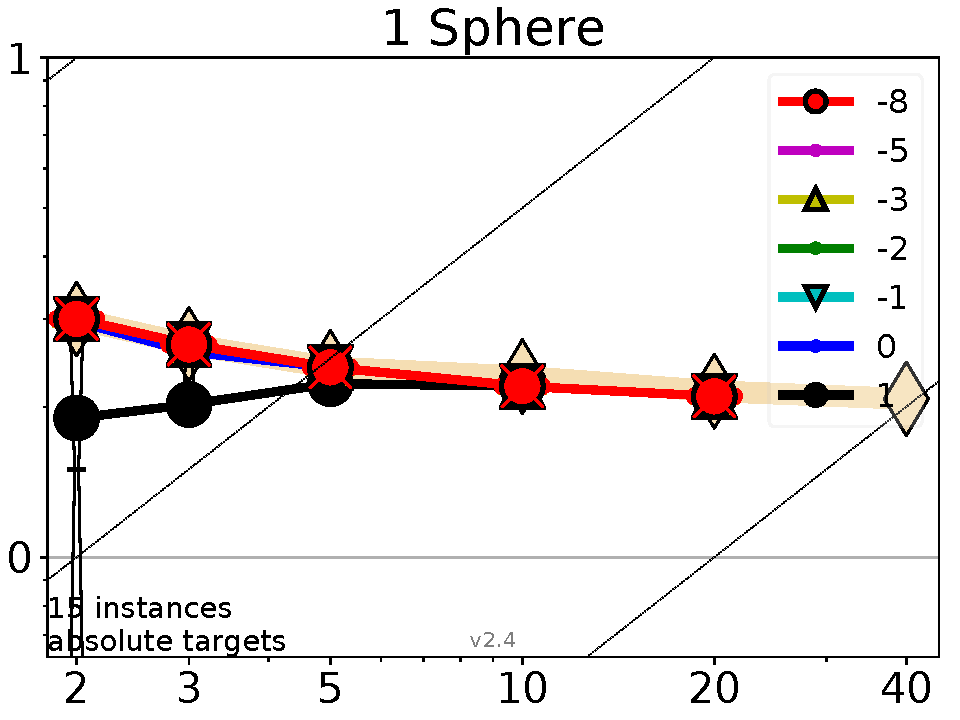
\includegraphics[width=0.24\textwidth]{ppfigdim_f001}&
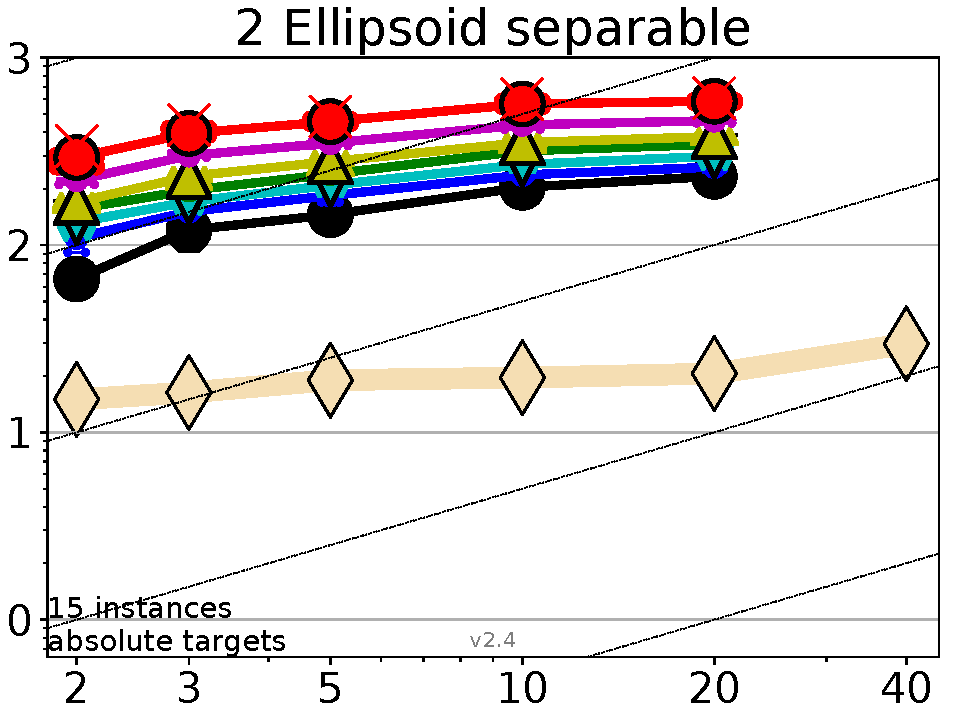
\includegraphics[width=0.24\textwidth]{ppfigdim_f002}&
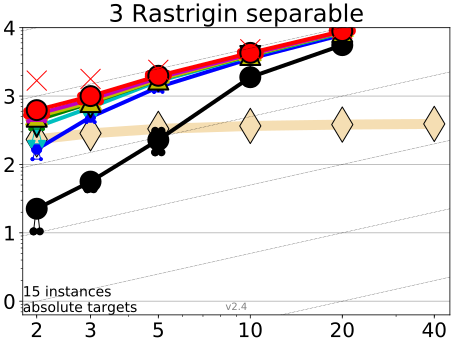
\includegraphics[width=0.24\textwidth]{ppfigdim_f003}&
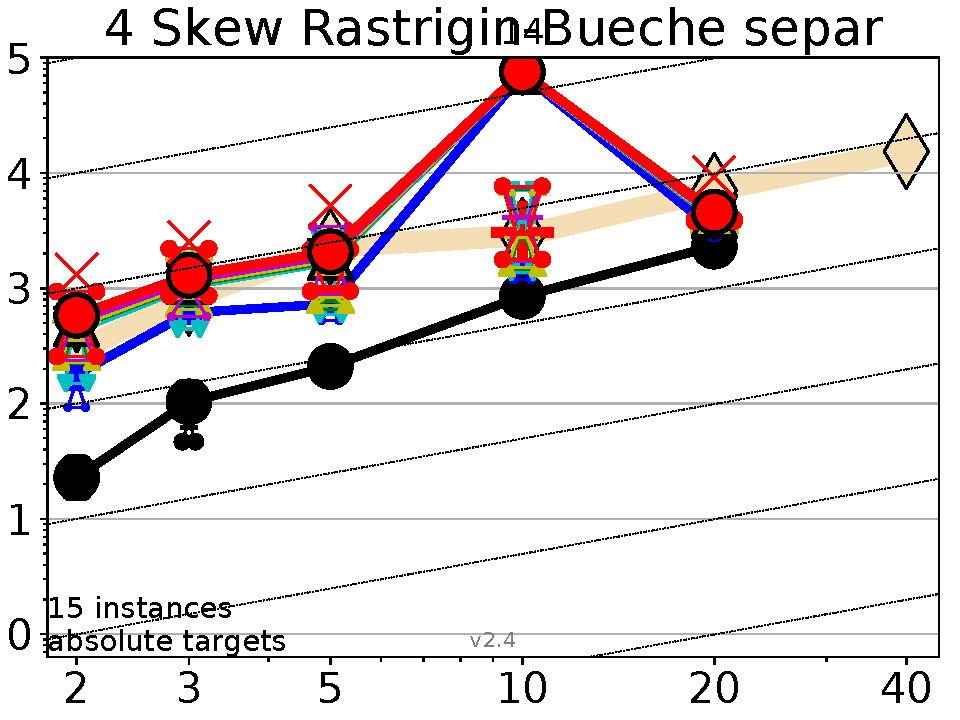
\includegraphics[width=0.24\textwidth]{ppfigdim_f004}\\[-1ex]
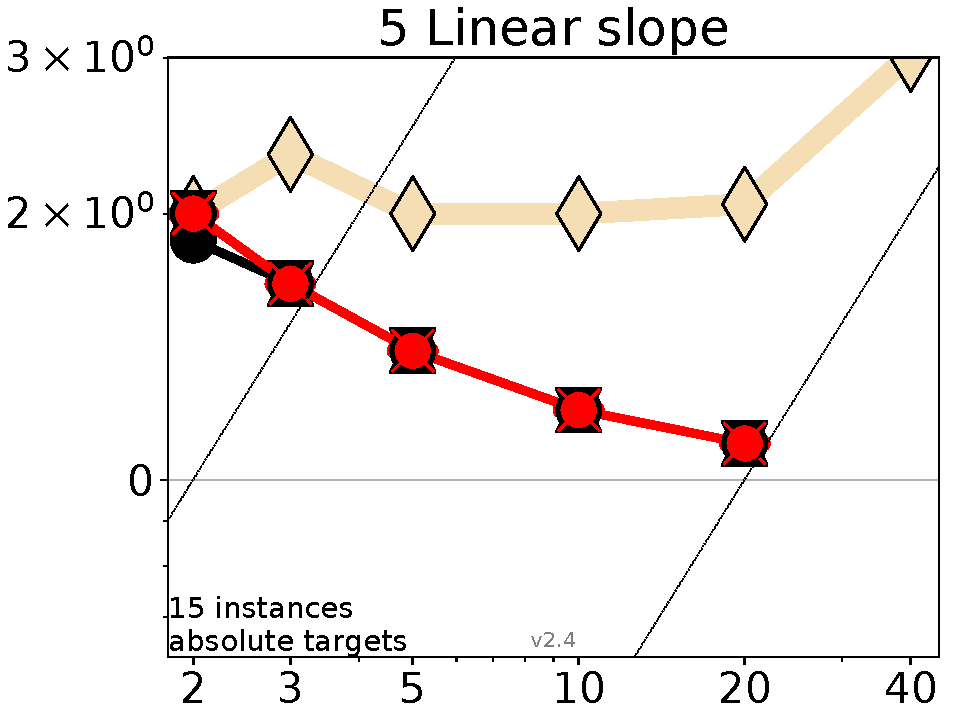
\includegraphics[width=0.24\textwidth]{ppfigdim_f005}&
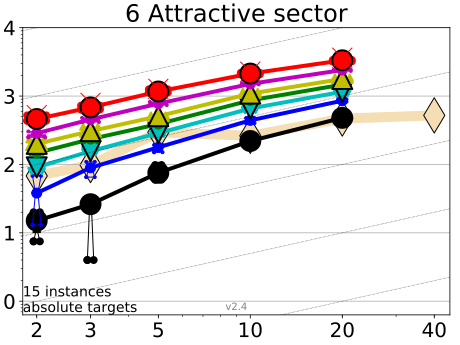
\includegraphics[width=0.24\textwidth]{ppfigdim_f006}&
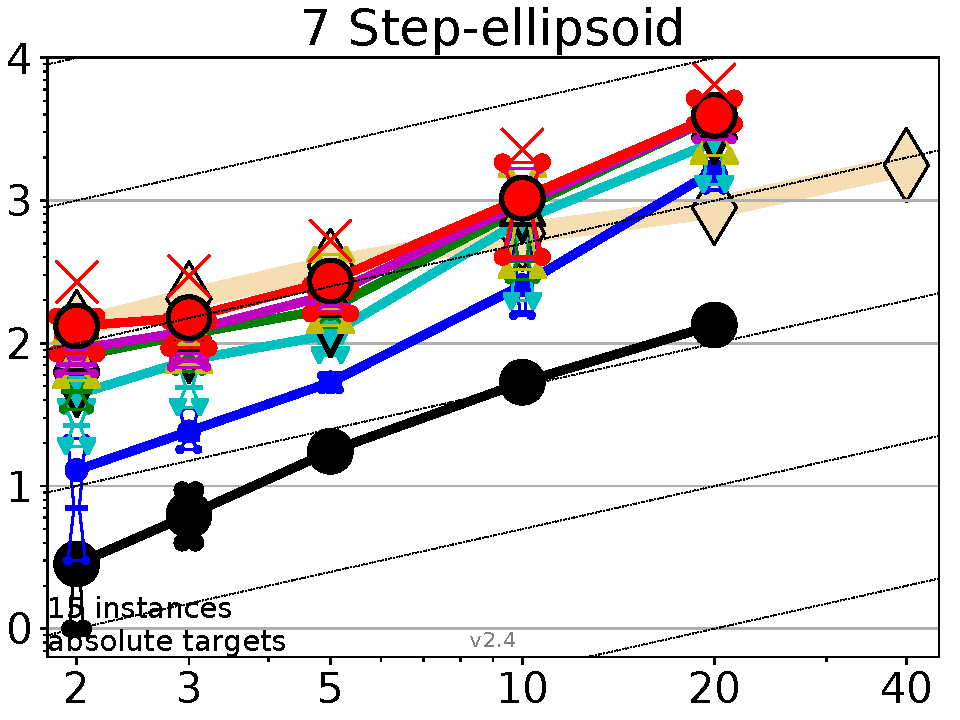
\includegraphics[width=0.24\textwidth]{ppfigdim_f007}&
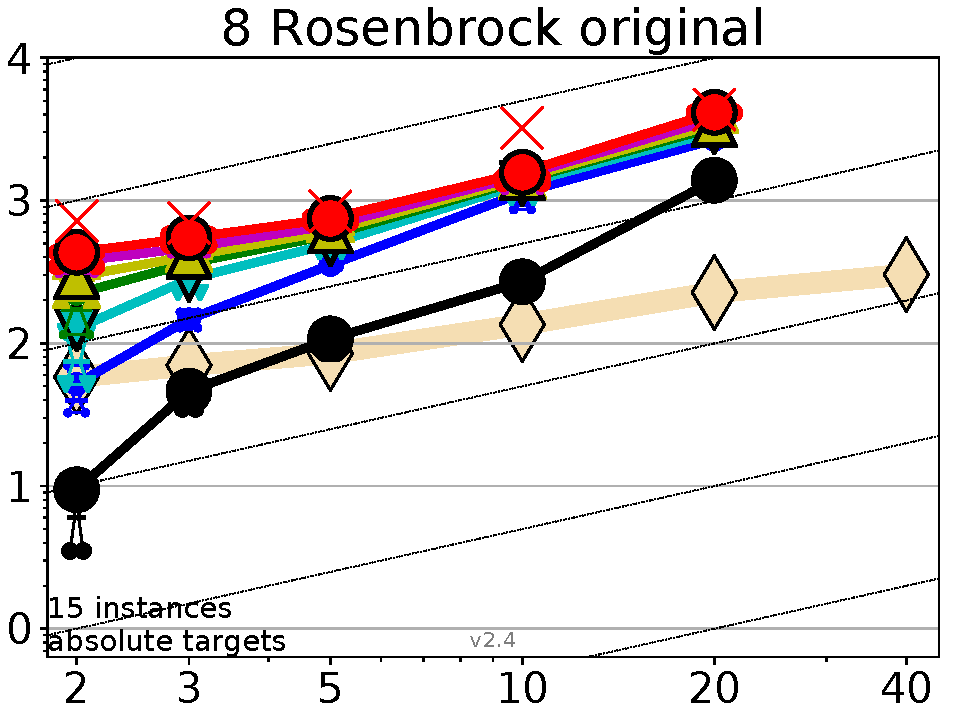
\includegraphics[width=0.24\textwidth]{ppfigdim_f008}\\[-1ex]
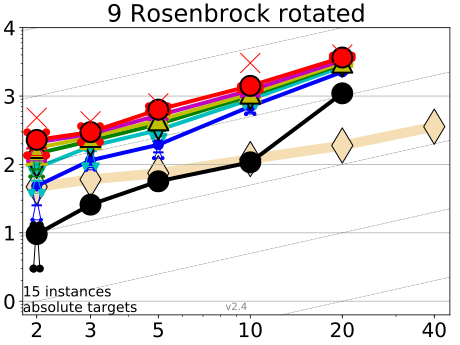
\includegraphics[width=0.24\textwidth]{ppfigdim_f009}&
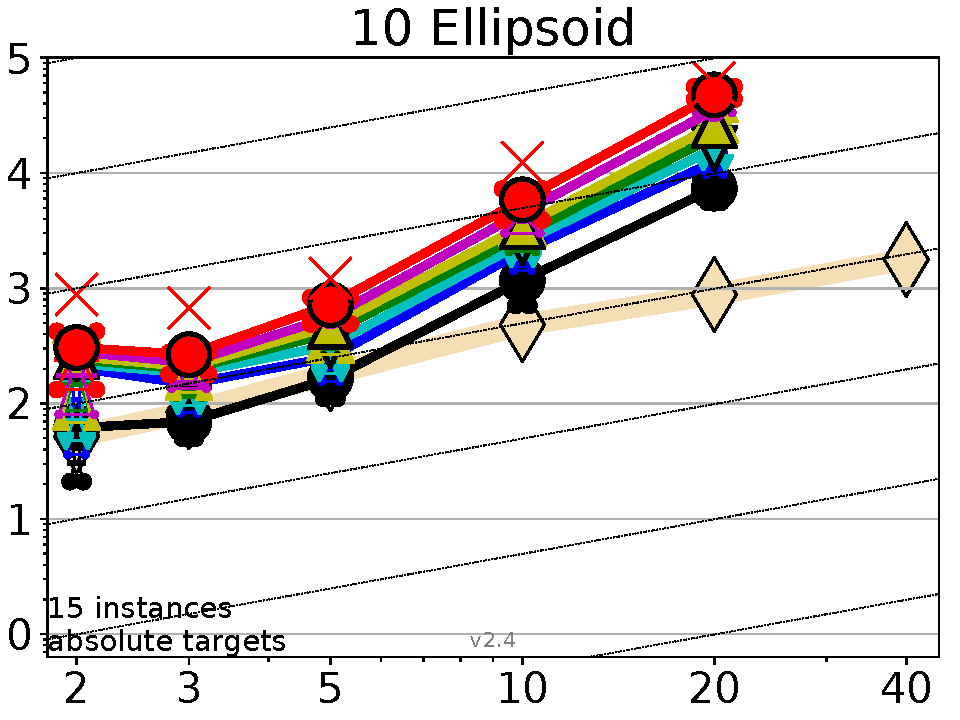
\includegraphics[width=0.24\textwidth]{ppfigdim_f010}&
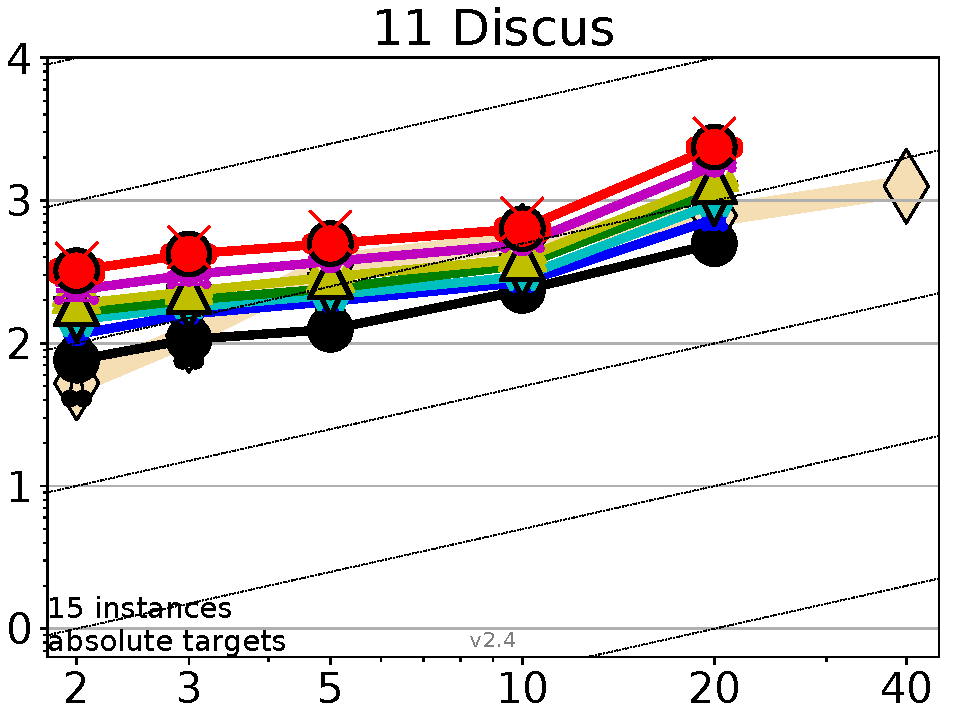
\includegraphics[width=0.24\textwidth]{ppfigdim_f011}&
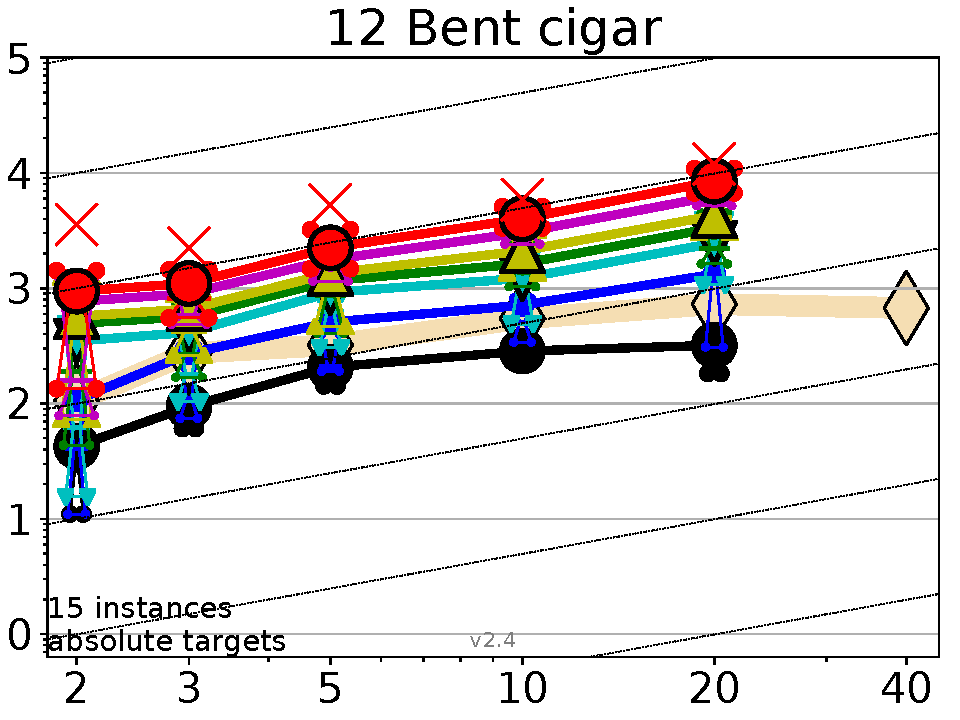
\includegraphics[width=0.24\textwidth]{ppfigdim_f012}\\[-1ex]
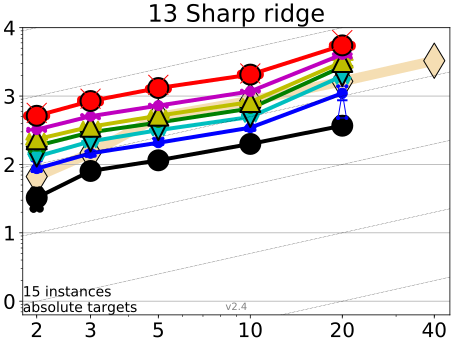
\includegraphics[width=0.24\textwidth]{ppfigdim_f013}&
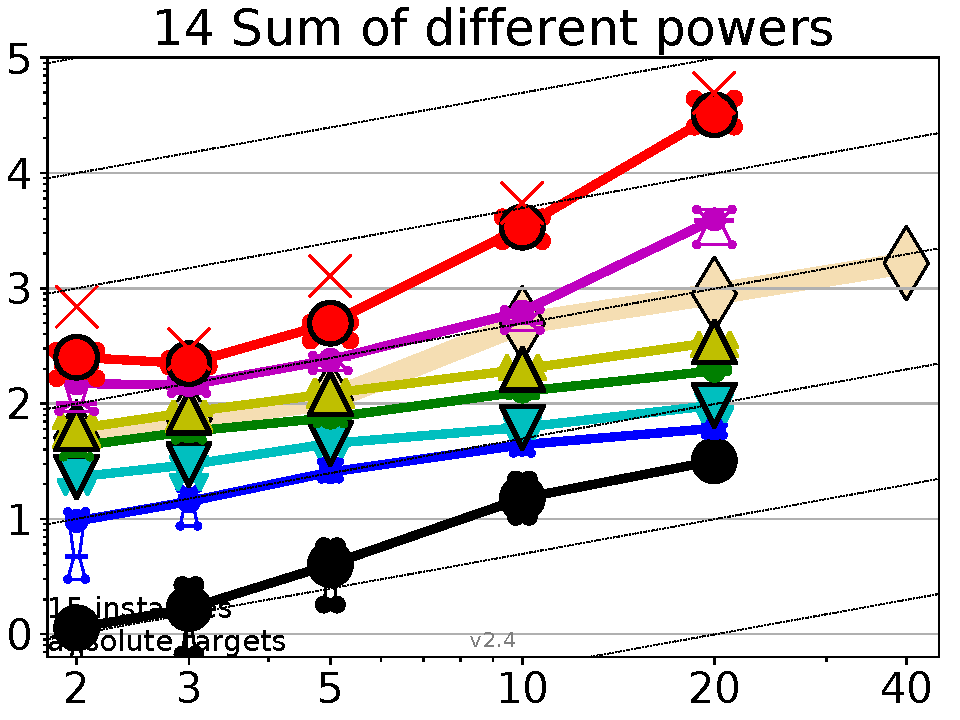
\includegraphics[width=0.24\textwidth]{ppfigdim_f014}&
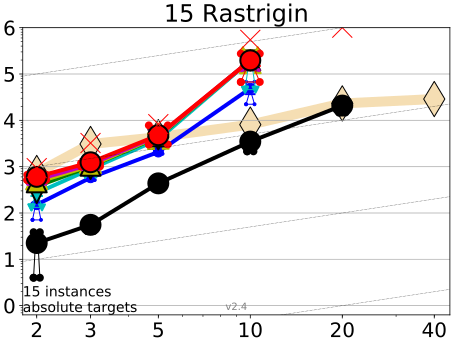
\includegraphics[width=0.24\textwidth]{ppfigdim_f015}&
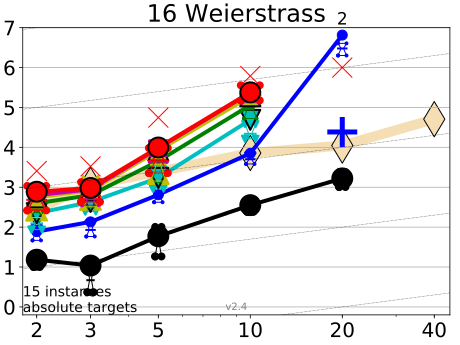
\includegraphics[width=0.24\textwidth]{ppfigdim_f016}\\[-1ex]
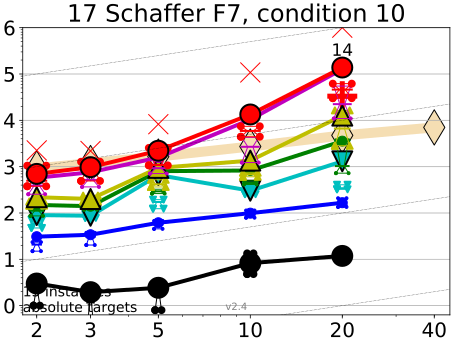
\includegraphics[width=0.24\textwidth]{ppfigdim_f017}&
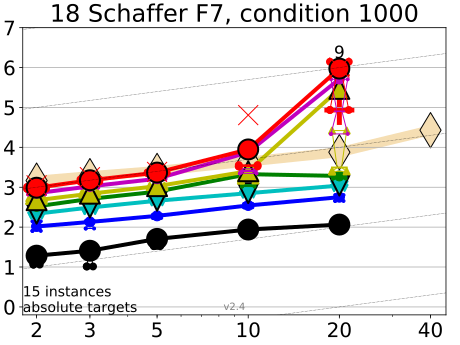
\includegraphics[width=0.24\textwidth]{ppfigdim_f018}&
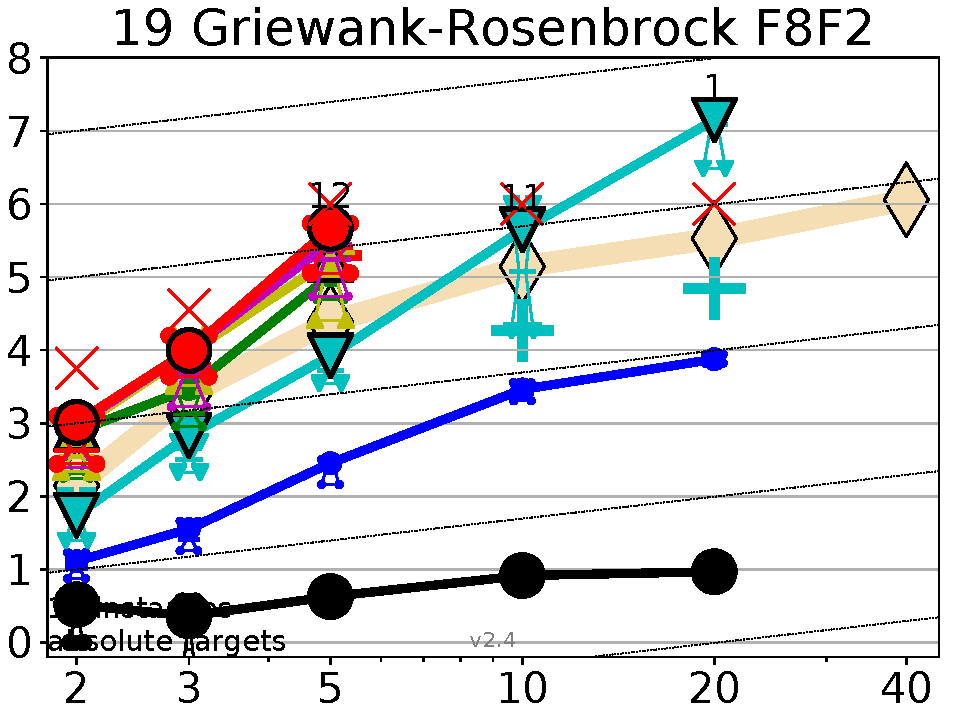
\includegraphics[width=0.24\textwidth]{ppfigdim_f019}&
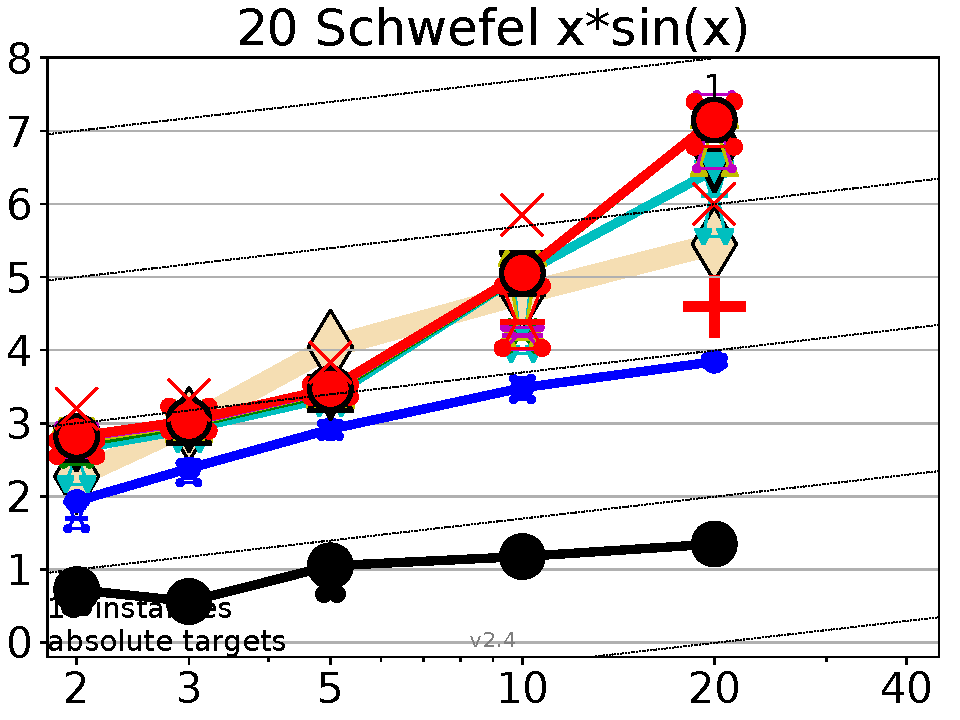
\includegraphics[width=0.24\textwidth]{ppfigdim_f020}\\[-1ex]
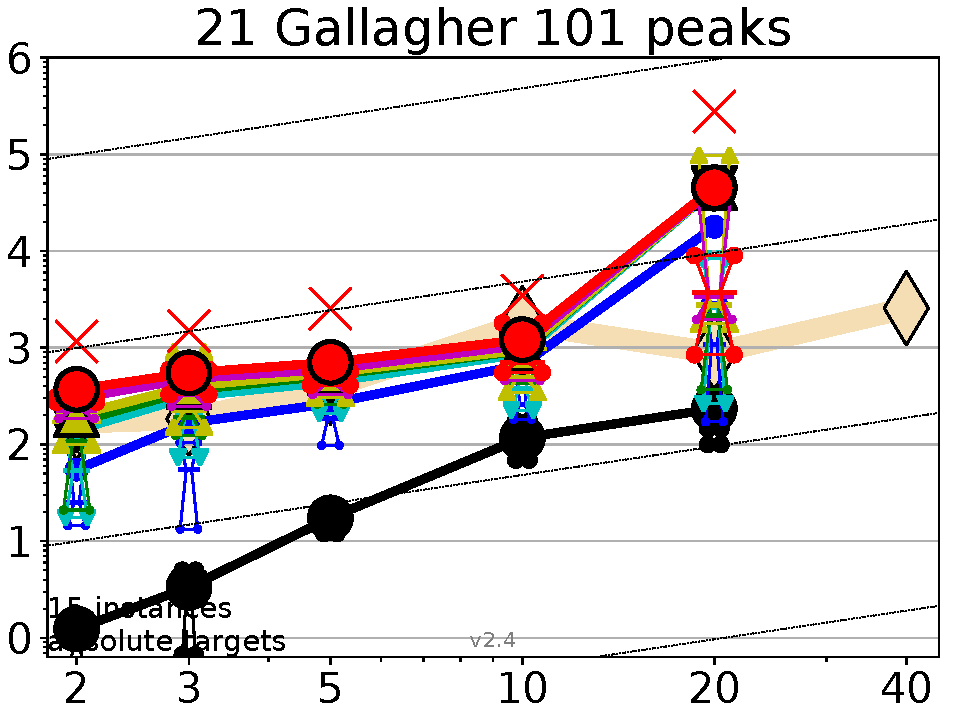
\includegraphics[width=0.24\textwidth]{ppfigdim_f021}&
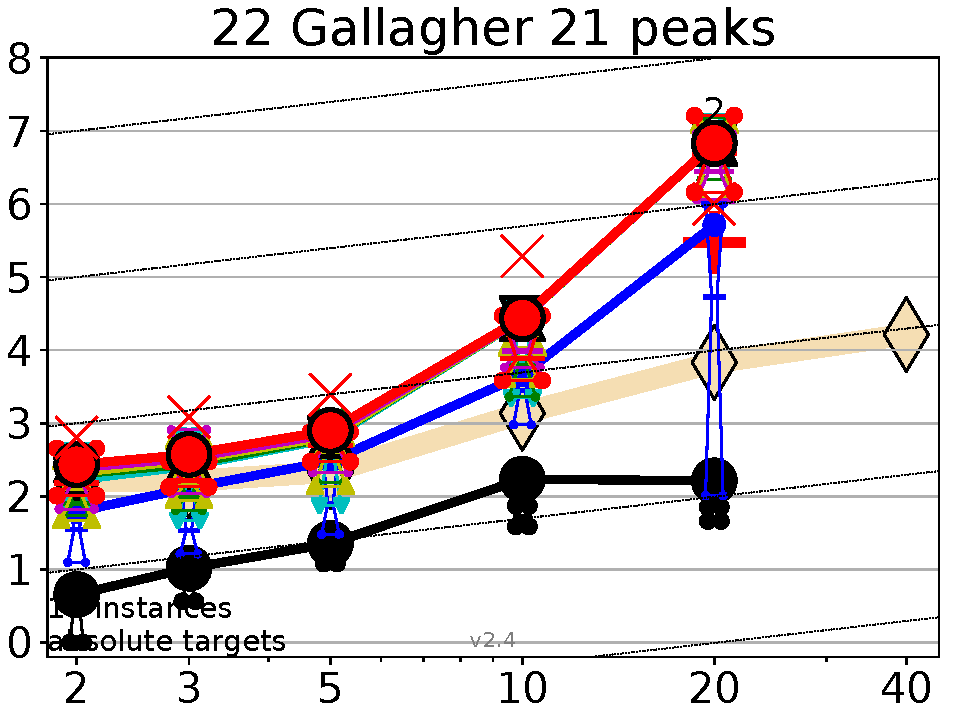
\includegraphics[width=0.24\textwidth]{ppfigdim_f022}&
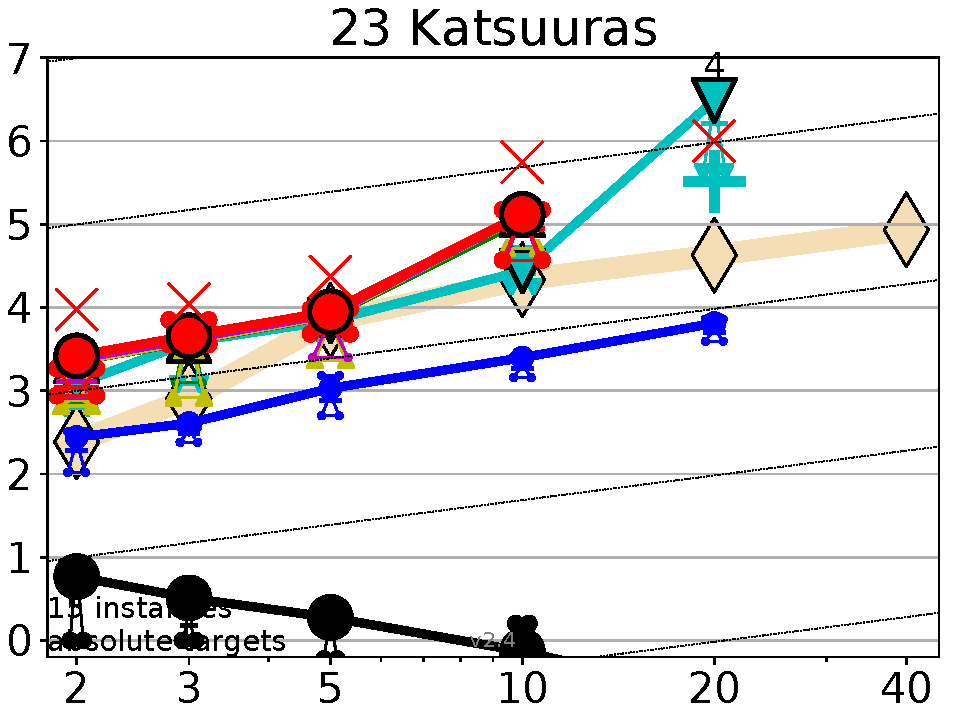
\includegraphics[width=0.24\textwidth]{ppfigdim_f023}&
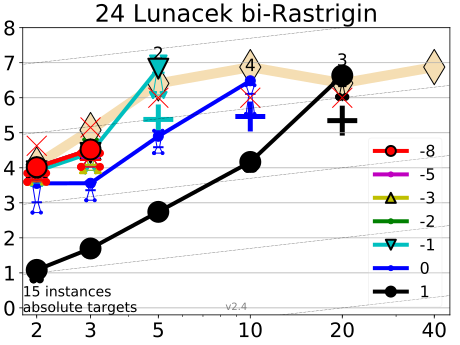
\includegraphics[width=0.24\textwidth]{ppfigdim_f024}
\end{tabular}
\vspace{-3ex}
 \caption{\label{fig:ERTgraphs}
 \bbobppfigdimlegend{$f_1$ and $f_{24}$}
 }
\end{figure*}



%%%%%%%%%%%%%%%%%%%%%%%%%%%%%%%%%%%%%%%%%%%%%%%%%%%%%%%%%%%%%%%%%%%%%%%%%%%%%%%
%%%%%%%%%%%%%%%%%%%%%%%%%%%%%%%%%%%%%%%%%%%%%%%%%%%%%%%%%%%%%%%%%%%%%%%%%%%%%%%

% ECDFs per function
%%%%%%%%%%%%%%%%%%%%%%%%%%%%%%%%%%%%%%%%%%%%%%%%%%%%%%%%%%%%%%%%%%%%%%%%%%%%%%%

\begin{figure*}
\centering
\begin{tabular}{l@{\hspace*{-0.00\textwidth}}l@{\hspace*{0.01\textwidth}}l@{\hspace*{-0.00\textwidth}}l}
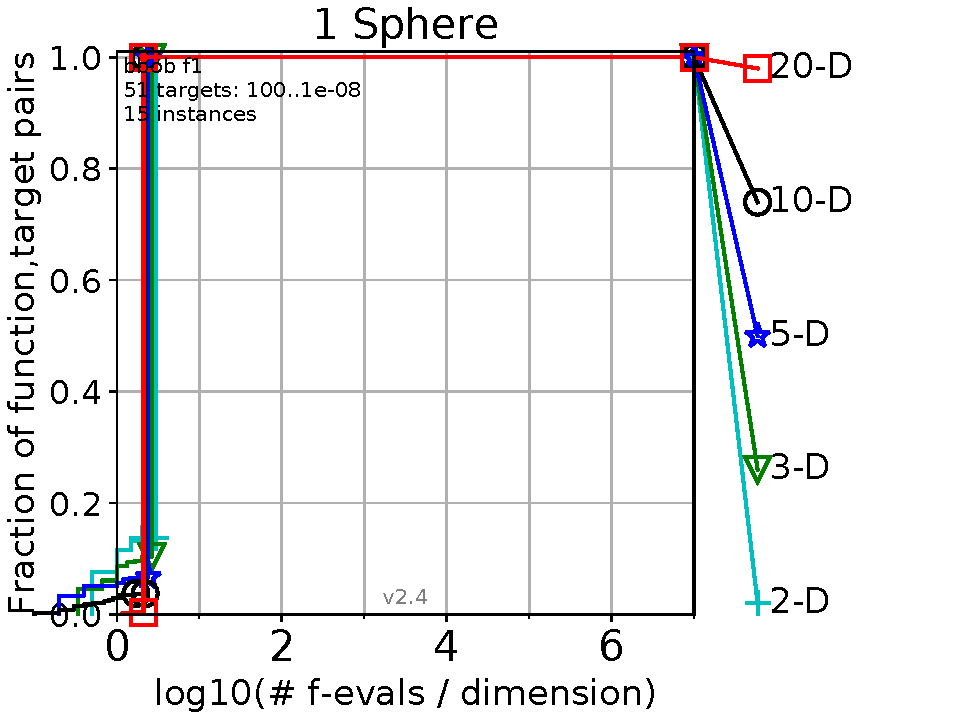
\includegraphics[width=0.24\textwidth]{pprldmany-single-functions/pprldmany_f001}&
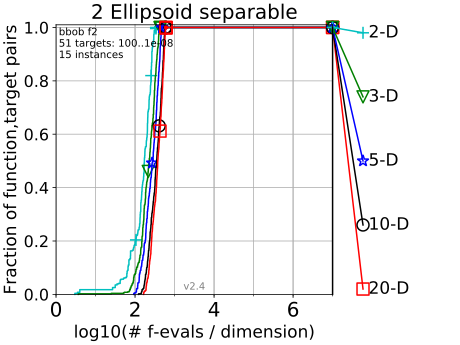
\includegraphics[width=0.24\textwidth]{pprldmany-single-functions/pprldmany_f002}&
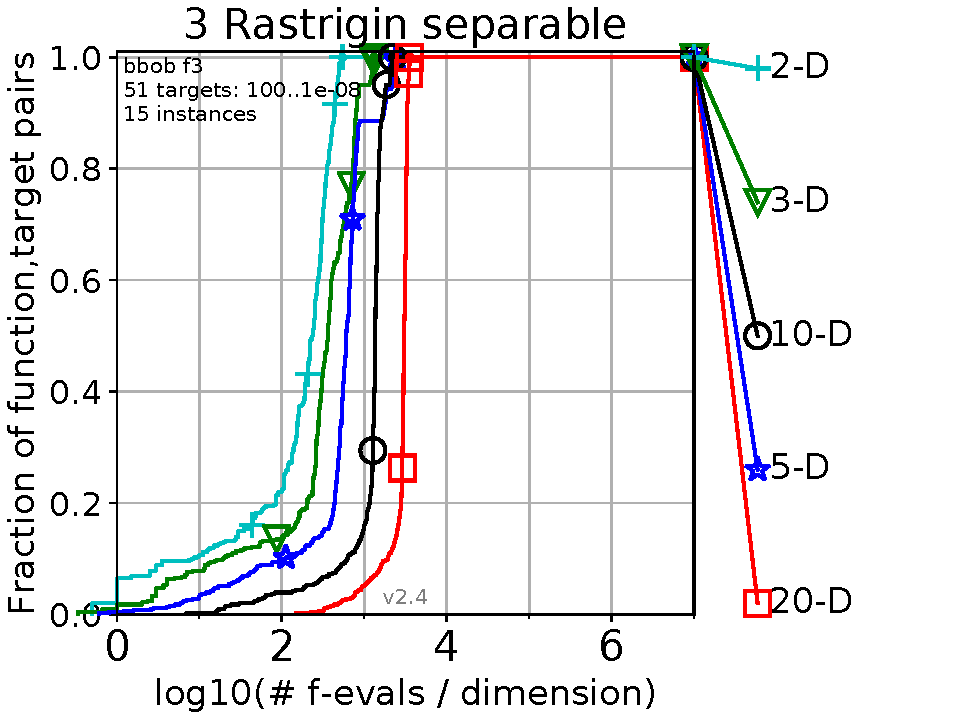
\includegraphics[width=0.24\textwidth]{pprldmany-single-functions/pprldmany_f003}&
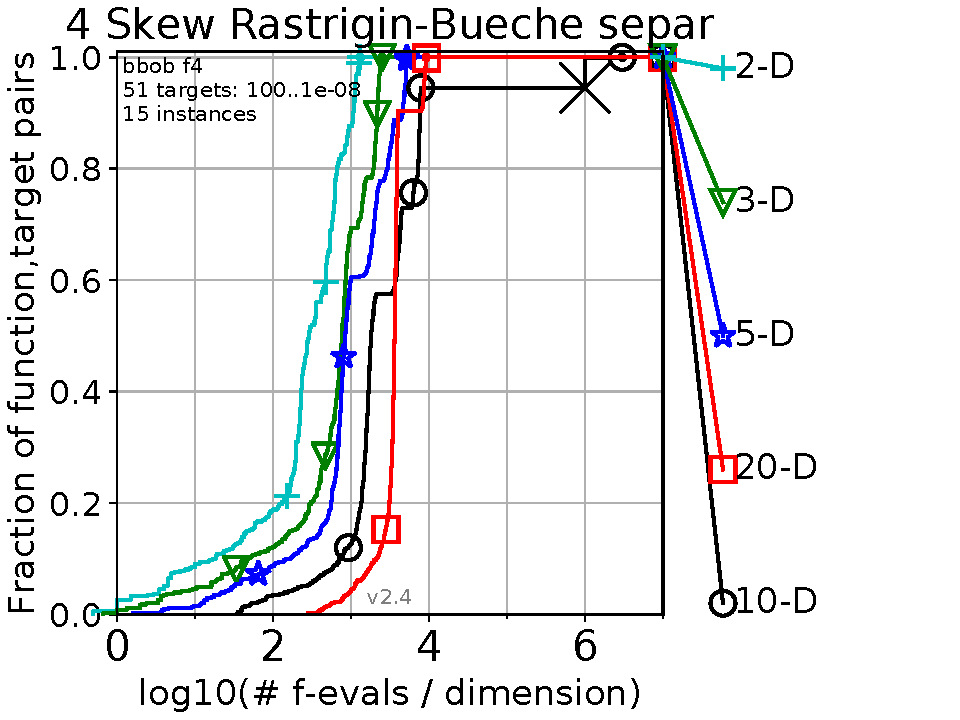
\includegraphics[width=0.24\textwidth]{pprldmany-single-functions/pprldmany_f004}\\[-0.2em]
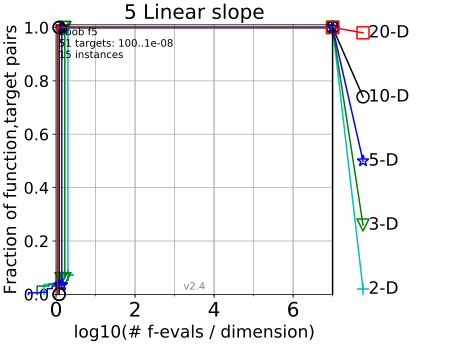
\includegraphics[width=0.24\textwidth]{pprldmany-single-functions/pprldmany_f005}&
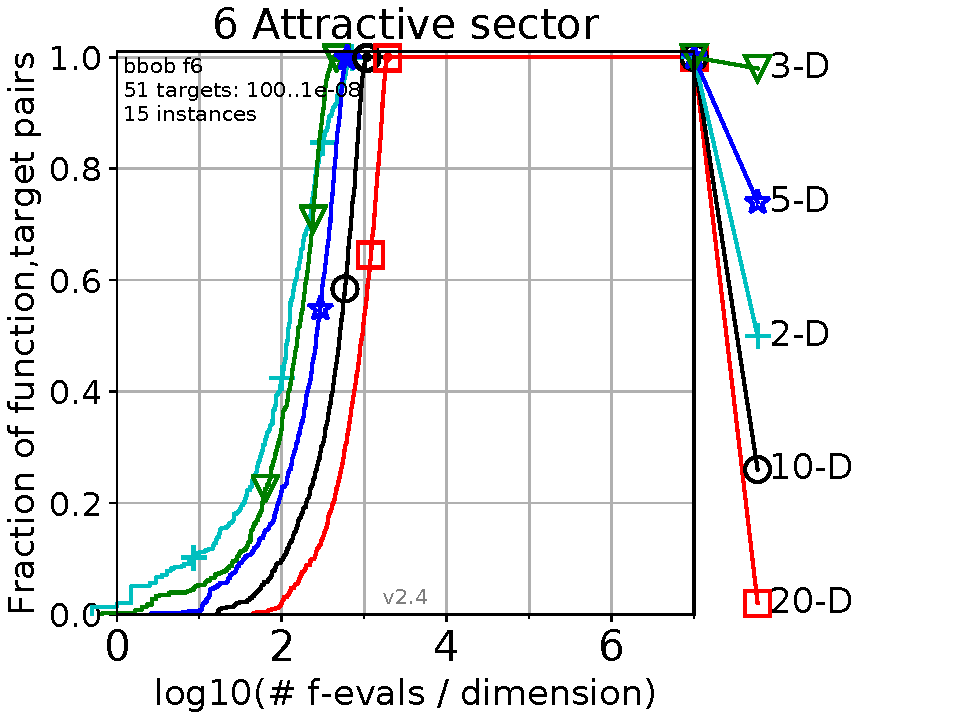
\includegraphics[width=0.24\textwidth]{pprldmany-single-functions/pprldmany_f006}&
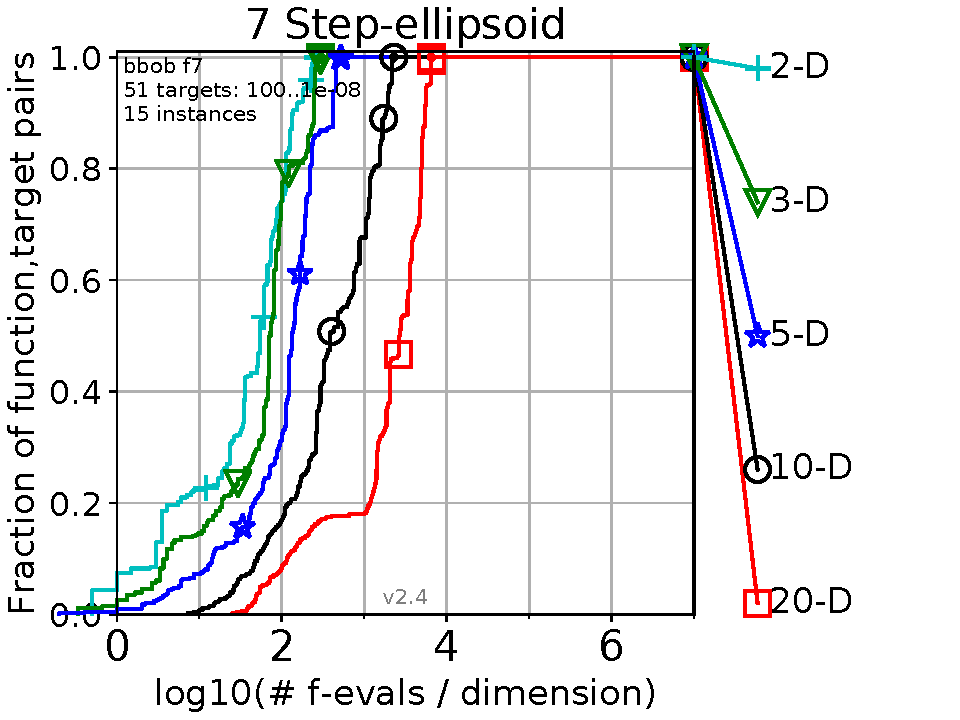
\includegraphics[width=0.24\textwidth]{pprldmany-single-functions/pprldmany_f007}&
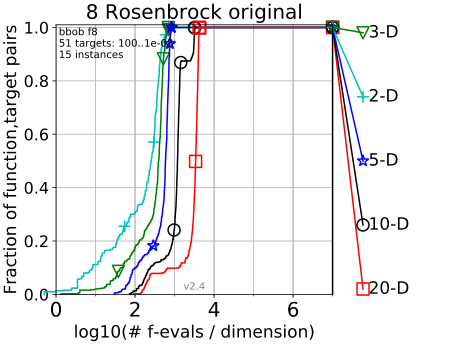
\includegraphics[width=0.24\textwidth]{pprldmany-single-functions/pprldmany_f008}\\[-0.2em]
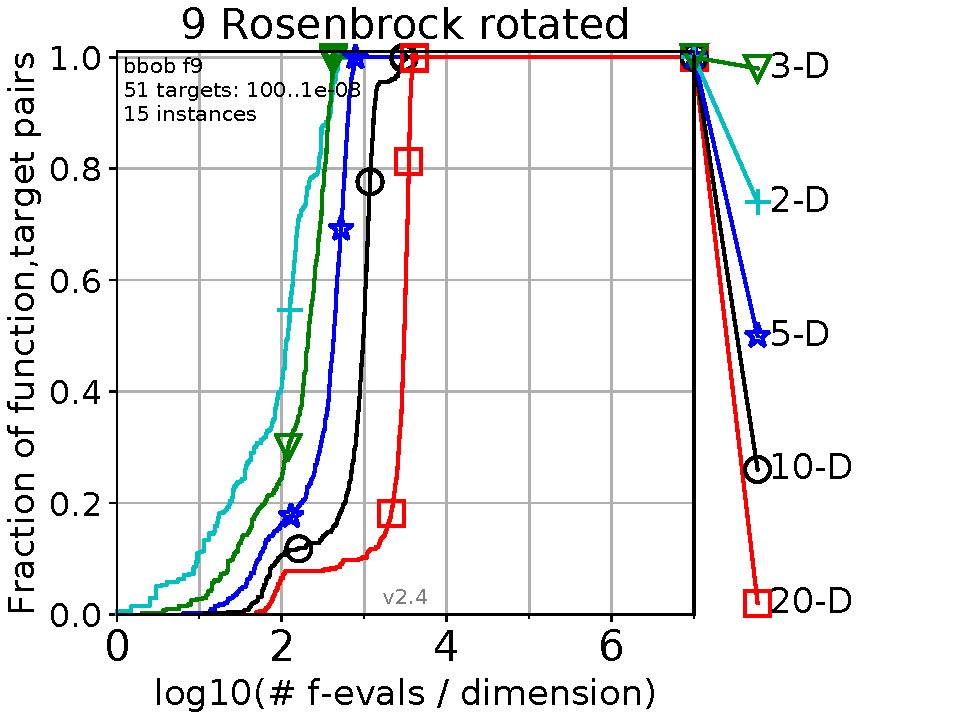
\includegraphics[width=0.24\textwidth]{pprldmany-single-functions/pprldmany_f009}&
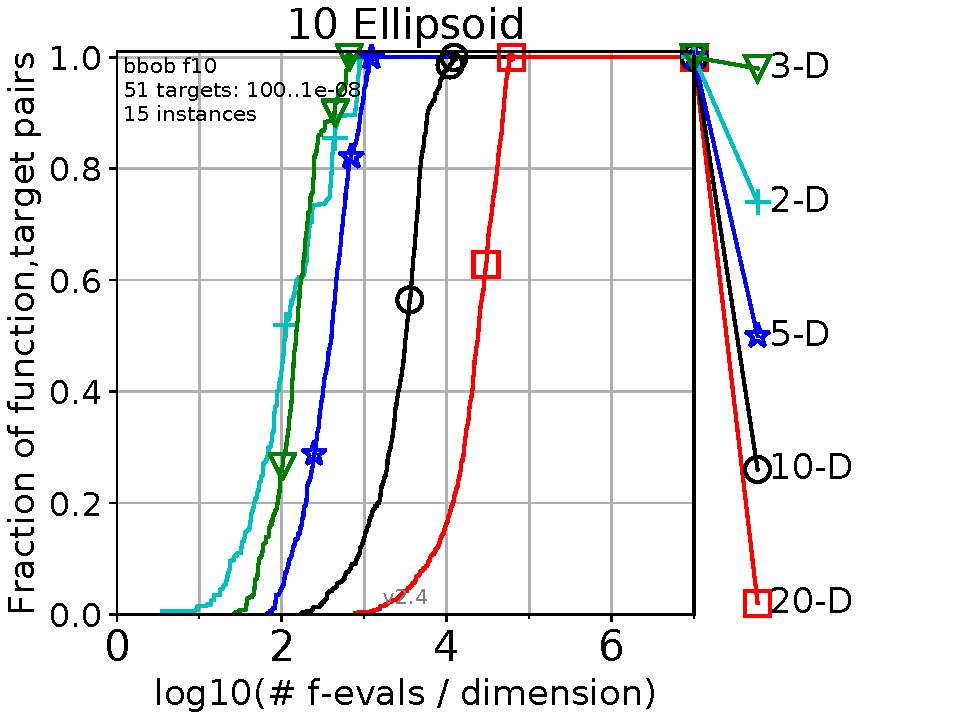
\includegraphics[width=0.24\textwidth]{pprldmany-single-functions/pprldmany_f010}&
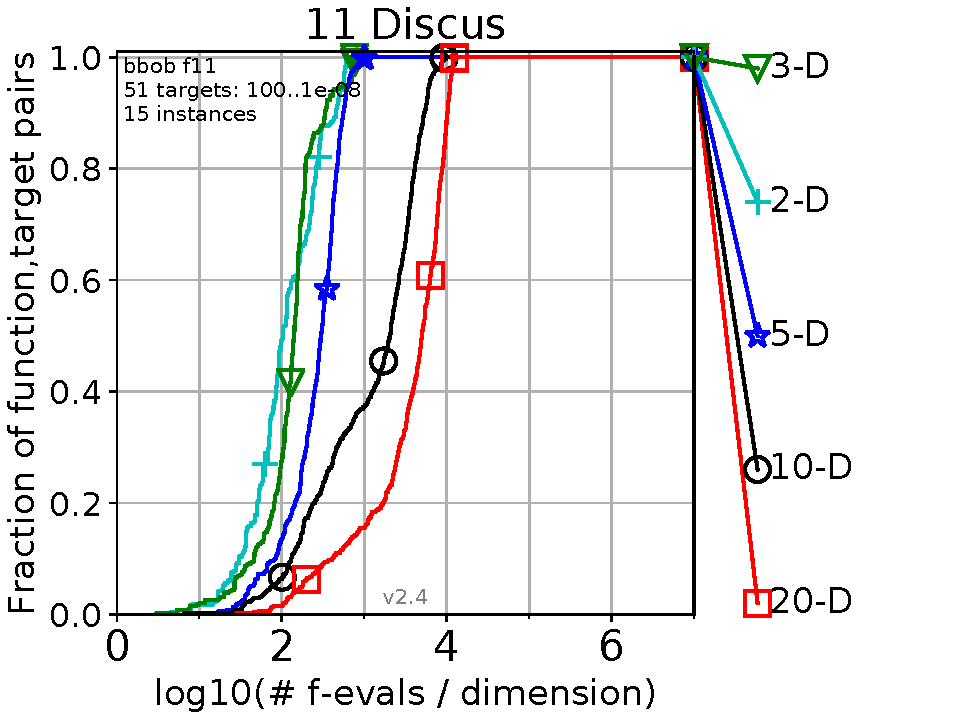
\includegraphics[width=0.24\textwidth]{pprldmany-single-functions/pprldmany_f011}&
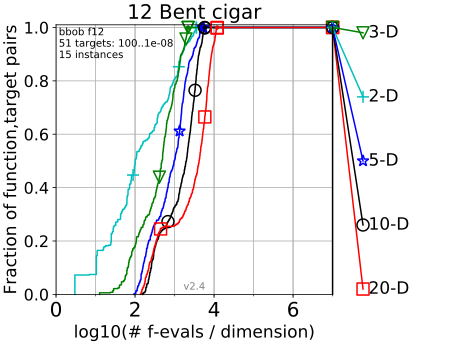
\includegraphics[width=0.24\textwidth]{pprldmany-single-functions/pprldmany_f012}\\[-0.2em]
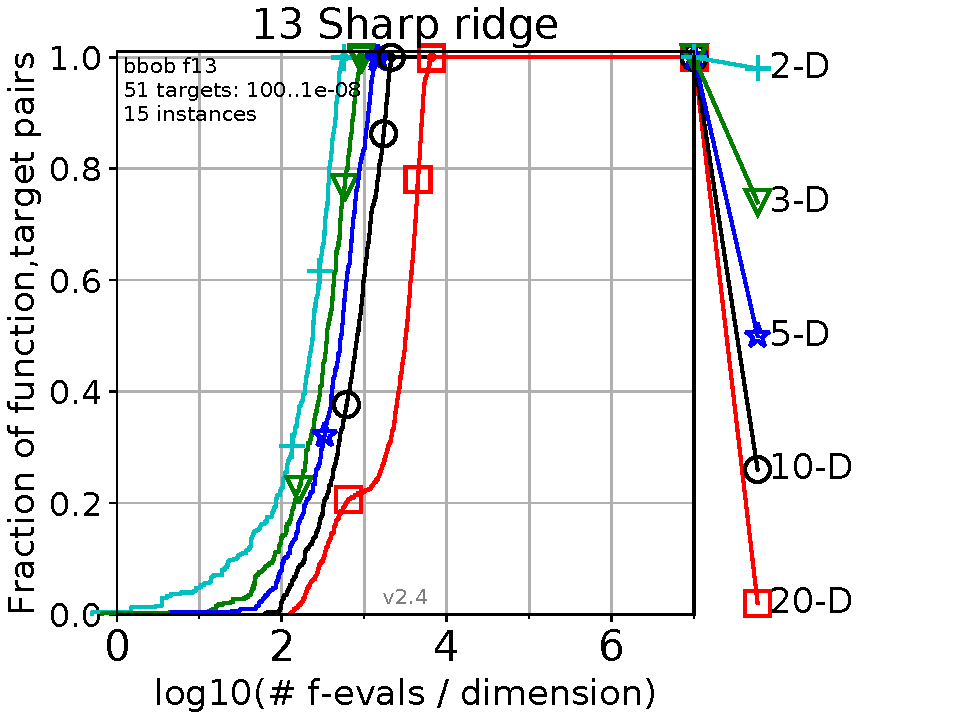
\includegraphics[width=0.24\textwidth]{pprldmany-single-functions/pprldmany_f013}&
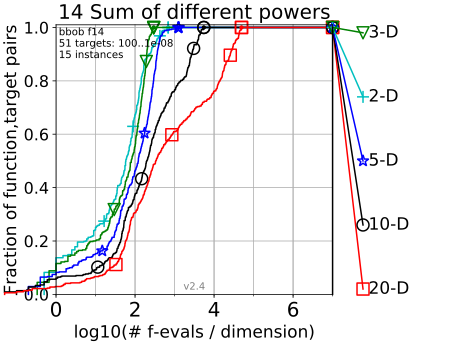
\includegraphics[width=0.24\textwidth]{pprldmany-single-functions/pprldmany_f014}&
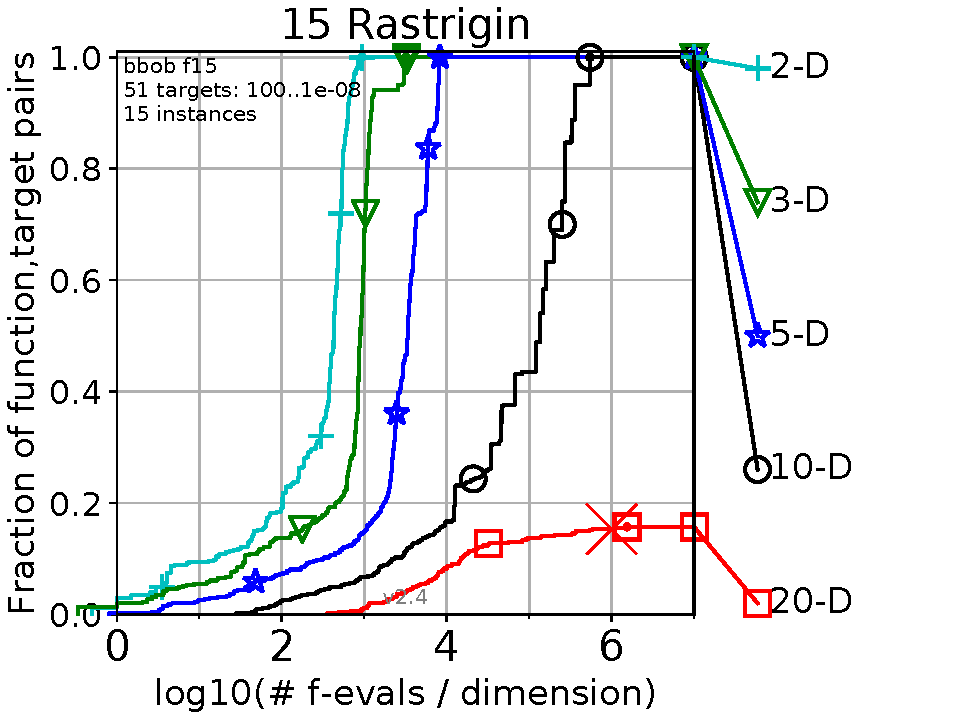
\includegraphics[width=0.24\textwidth]{pprldmany-single-functions/pprldmany_f015}&
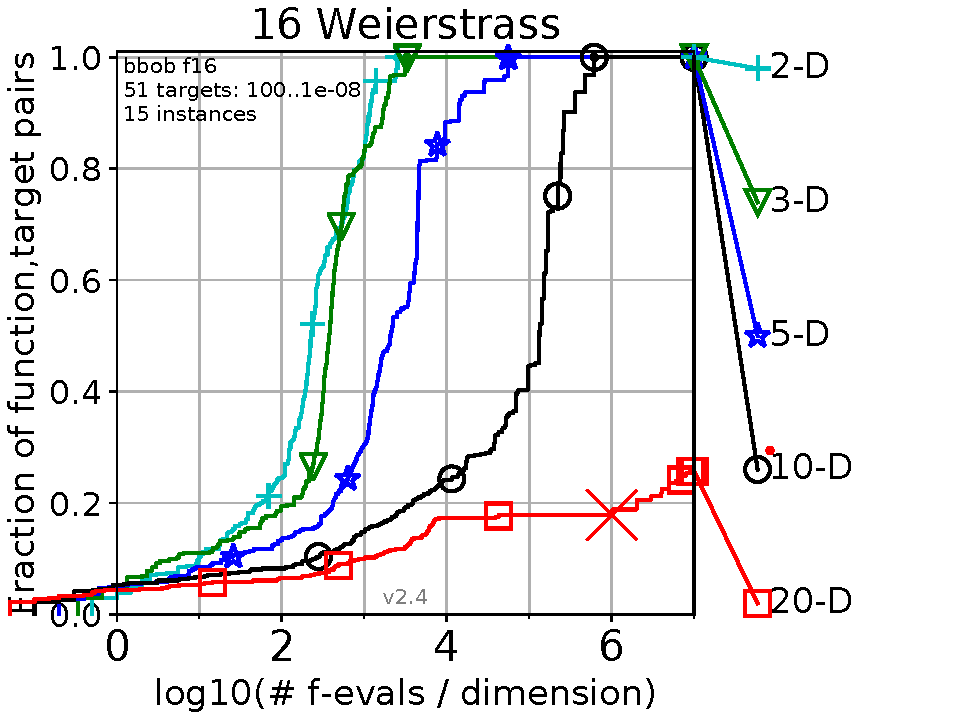
\includegraphics[width=0.24\textwidth]{pprldmany-single-functions/pprldmany_f016}\\[-0.2em]
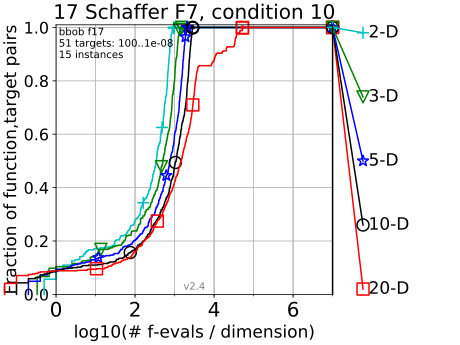
\includegraphics[width=0.24\textwidth]{pprldmany-single-functions/pprldmany_f017}&
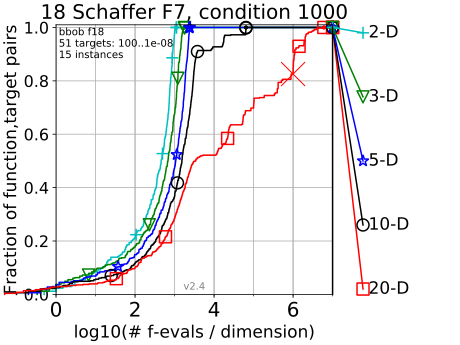
\includegraphics[width=0.24\textwidth]{pprldmany-single-functions/pprldmany_f018}&
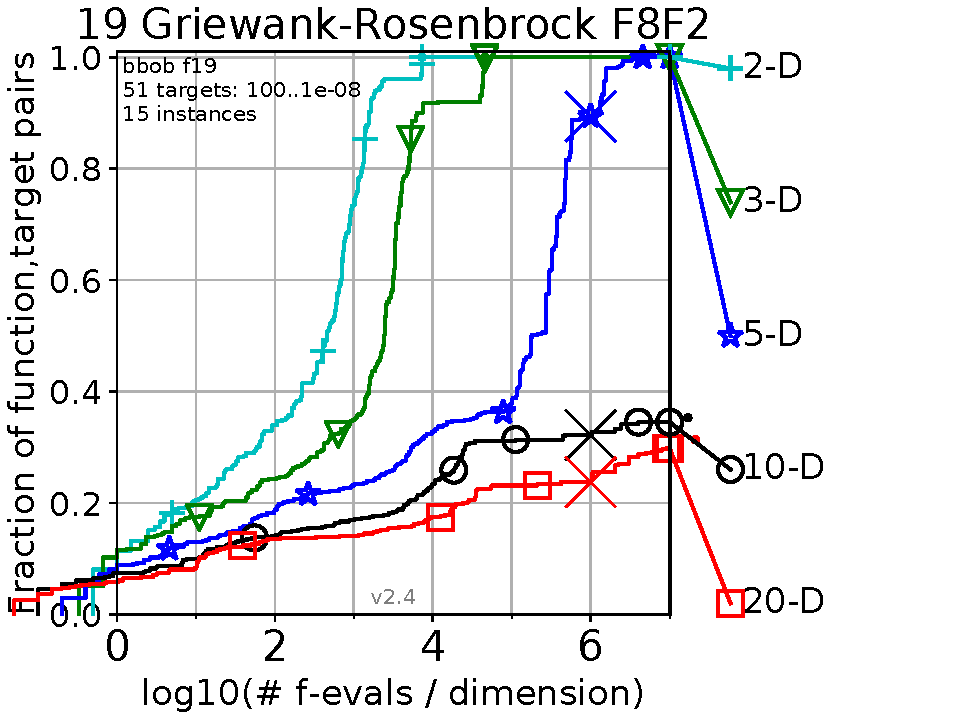
\includegraphics[width=0.24\textwidth]{pprldmany-single-functions/pprldmany_f019}&
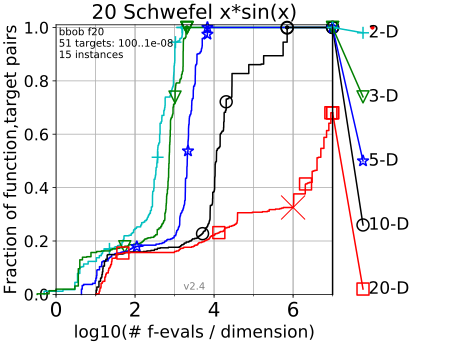
\includegraphics[width=0.24\textwidth]{pprldmany-single-functions/pprldmany_f020}\\[-0.2em]
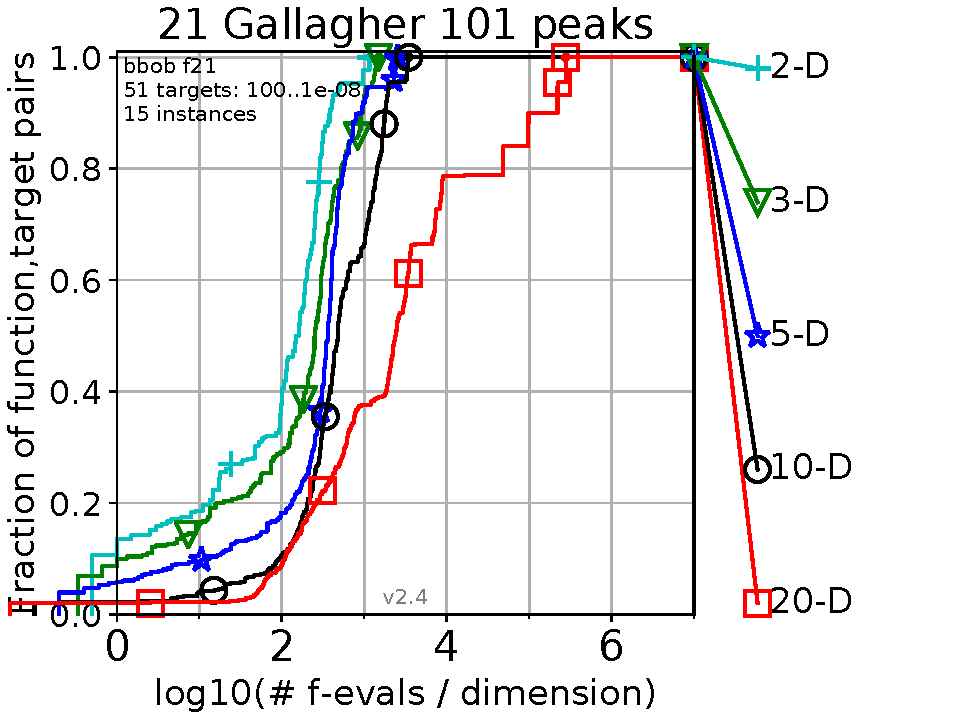
\includegraphics[width=0.24\textwidth]{pprldmany-single-functions/pprldmany_f021}&
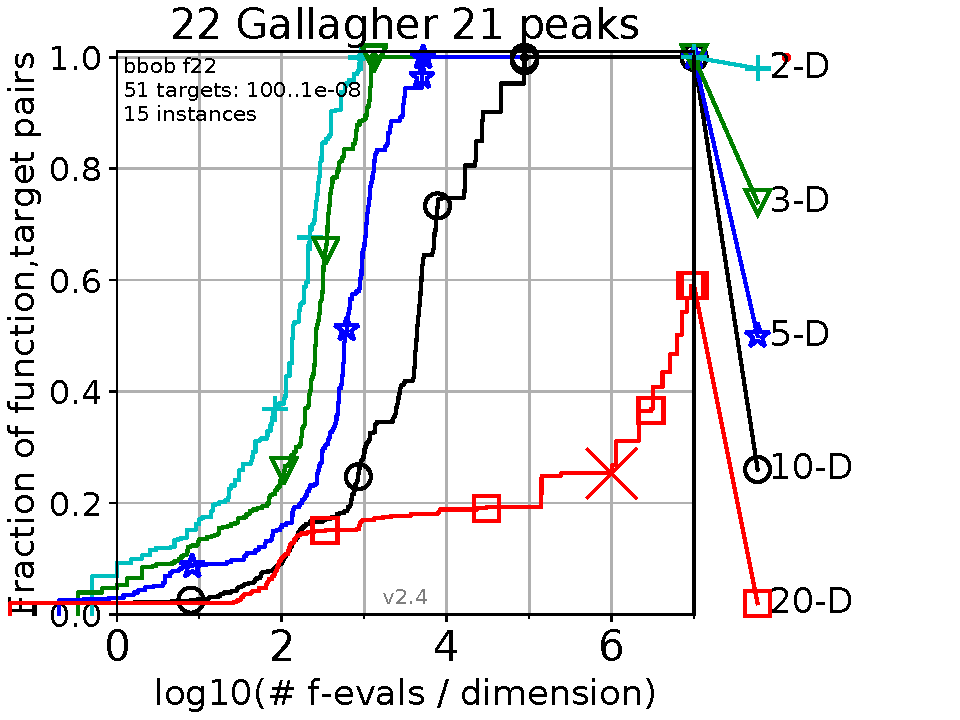
\includegraphics[width=0.24\textwidth]{pprldmany-single-functions/pprldmany_f022}&
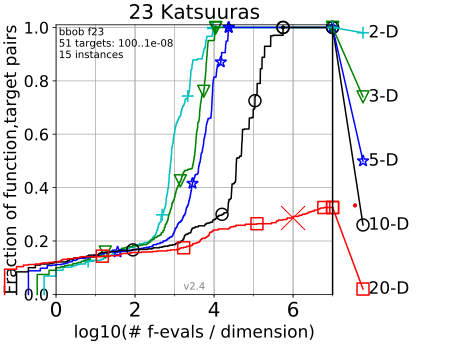
\includegraphics[width=0.24\textwidth]{pprldmany-single-functions/pprldmany_f023}&
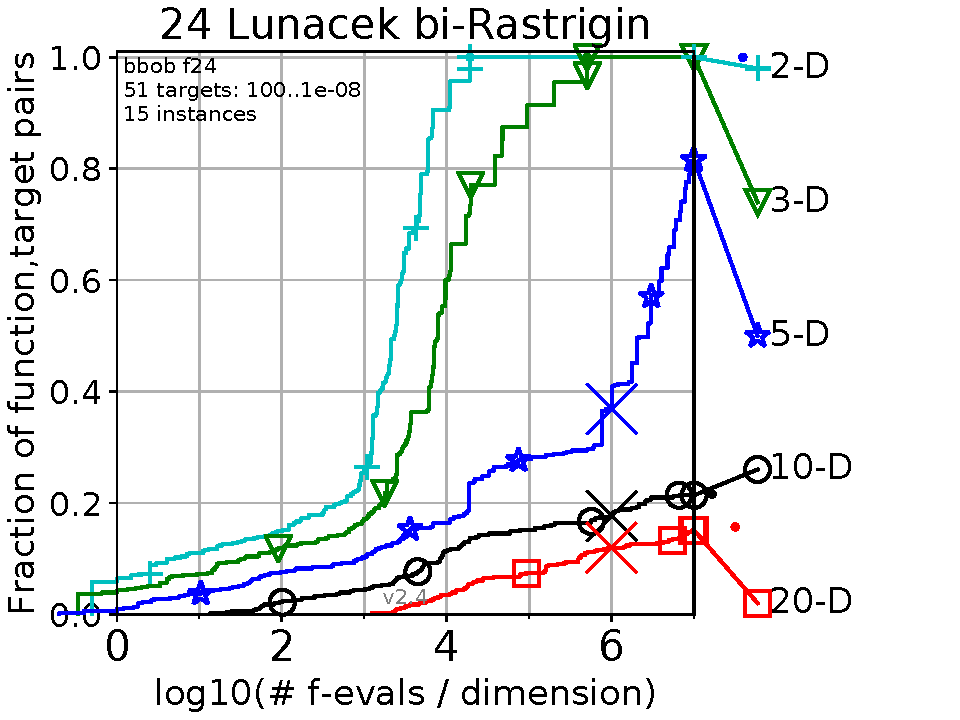
\includegraphics[width=0.24\textwidth]{pprldmany-single-functions/pprldmany_f024}
\vspace*{-1ex}
\end{tabular}
 \caption{\label{fig:ECDFsingleOne}
	\bbobecdfcaptionsinglefunctionssingledim{$\!\!$s 5 to 160}
}
\end{figure*}




%%%%%%%%%%%%%%%%%%%%%%%%%%%%%%%%%%%%%%%%%%%%%%%%%%%%%%%%%%%%%%%%%%%%%%%%%%%%%%%
%%%%%%%%%%%%%%%%%%%%%%%%%%%%%%%%%%%%%%%%%%%%%%%%%%%%%%%%%%%%%%%%%%%%%%%%%%%%%%%%
%
%% ERT loss ratios (figure and table) [not yet available]
%
%%%%%%%%%%%%%%%%%%%%%%%%%%%%%%%%%%%%%%%%%%%%%%%%%%%%%%%%%%%%%%%%%%%%%%%%%%%%%%%%
%\begin{figure}
%\centering
%\parbox{0.48\columnwidth}{\centering 10-D}\hfill
%\parbox{0.48\columnwidth}{\centering 40-D}\\
%\includegraphics[width=0.48\columnwidth]{pplogloss_10D_noiselessall}\hfill
%\includegraphics[width=0.48\columnwidth]{pplogloss_40D_noiselessall}\\[2ex]
%%
%\input{\bbobdatapath\algfolder pploglosstable_10D_noiselessall}\\
%\input{\bbobdatapath\algfolder pploglosstable_40D_noiselessall}
%\caption{\label{tab:ERTloss}%
%\bbobloglosstablecaption{}
%}
%\end{figure}


%%%%%%%%%%%%%%%%%%%%%%%%%%%%%%%%%%%%%%%%%%%%%%%%%%%%%%%%%%%%%%%%%%%%%%%%%%%%%%%
%%%%%%%%%%%%%%%%%%%%%%%%%%%%%%%%%%%%%%%%%%%%%%%%%%%%%%%%%%%%%%%%%%%%%%%%%%%%%%%%
%
%% ERT loss ratios per function group [not yet available]
%
%%%%%%%%%%%%%%%%%%%%%%%%%%%%%%%%%%%%%%%%%%%%%%%%%%%%%%%%%%%%%%%%%%%%%%%%%%%%%%%%
%\begin{figure}
%\begin{tabular}{@{}l@{}@{}l@{}}
%\multicolumn{1}{c}{10-D} & \multicolumn{1}{c}{40-D}\\
%%\rot{all functions}
%%\hspace*{-2mm}
%\rot[2.8]{separable fcts}
%\hspace*{-1.4mm}
%\includegraphics[width=0.24\textwidth]{pplogloss_10D_separ} &
%\includegraphics[width=0.24\textwidth]{pplogloss_40D_separ}\\
%\rot[2.7]{moderate fcts}
%\hspace*{-1.4mm}
%\includegraphics[width=0.24\textwidth]{pplogloss_10D_lcond} &
%\includegraphics[width=0.24\textwidth]{pplogloss_40D_lcond}\\
%\rot[1.9]{ill-conditioned fcts}
%\hspace*{-1.35mm}
%\includegraphics[width=0.24\textwidth]{pplogloss_10D_hcond} &
%\includegraphics[width=0.24\textwidth]{pplogloss_40D_hcond}\\
%\rot[2.5]{multi-modal fcts}
%\hspace*{-1.3mm}
%\includegraphics[width=0.24\textwidth]{pplogloss_10D_multi} &
%\includegraphics[width=0.24\textwidth]{pplogloss_40D_multi}\\
%\rot[1.6]{weak structure fcts}
%\hspace*{-1.4mm}
%\includegraphics[width=0.24\textwidth]{pplogloss_10D_mult2} &
%\includegraphics[width=0.24\textwidth]{pplogloss_40D_mult2}
%\vspace*{-0.5ex}
%\end{tabular}
% \caption{\label{fig:ERTlogloss}%
%\bbobloglossfigurecaption{}
%}
%\end{figure}

%%%%%%%%%%%%%%%%%%%%%%%%%%%%%%%%%%%%%%%%%%%%%%%%%%%%%%%%%%%%%%%%%%%%%%%%%%%%%%%

%%%%%%%%%%%%%%%%%%%%%%%%%%%%%%%%%%%%%%%%%%%%%%%%%%%%%%%%%%%%%%%%%%%%%%%%%%%%%%%
 
% Table showing the expected runtime (ERT in number of function
% evaluations) divided by the best ERT measured during BBOB-2009 (given in the
% first row of each cell) for functions $f_1$--$f_{24} for dimension 10$.

%%%%%%%%%%%%%%%%%%%%%%%%%%%%%%%%%%%%%%%%%%%%%%%%%%%%%%%%%%%%%%%%%%%%%%%%%%%%%%%

\begin{table*}\tiny
%\hfill10-D\hfill~\\[1ex]
{\normalsize \color{red}
\ifthenelse{\isundefined{\algorithmG}}{}{more than 6 algorithms: please split the tables below by hand until it fits to the page limits}
}
\mbox{\begin{minipage}[t]{0.499\textwidth}\tiny
\centering
\pptableheader 

\input{\bbobdatapath\algfolder pptable_f001_10D} 

\input{\bbobdatapath\algfolder pptable_f002_10D}

\input{\bbobdatapath\algfolder pptable_f003_10D}

\input{\bbobdatapath\algfolder pptable_f004_10D}

\input{\bbobdatapath\algfolder pptable_f005_10D}

\input{\bbobdatapath\algfolder pptable_f006_10D}

\input{\bbobdatapath\algfolder pptable_f007_10D}

\input{\bbobdatapath\algfolder pptable_f008_10D}

\input{\bbobdatapath\algfolder pptable_f009_10D}

\input{\bbobdatapath\algfolder pptable_f010_10D}

\input{\bbobdatapath\algfolder pptable_f011_10D}

\input{\bbobdatapath\algfolder pptable_f012_10D}

\pptablefooter

\end{minipage}
\hspace{0.002\textwidth}
\begin{minipage}[t]{0.499\textwidth}\tiny
\centering

\pptableheader 

\input{\bbobdatapath\algfolder pptable_f013_10D}

\input{\bbobdatapath\algfolder pptable_f014_10D}

\input{\bbobdatapath\algfolder pptable_f015_10D}

\input{\bbobdatapath\algfolder pptable_f016_10D}

\input{\bbobdatapath\algfolder pptable_f017_10D}

\input{\bbobdatapath\algfolder pptable_f018_10D}

\input{\bbobdatapath\algfolder pptable_f019_10D}

\input{\bbobdatapath\algfolder pptable_f020_10D}

\input{\bbobdatapath\algfolder pptable_f021_10D}

\input{\bbobdatapath\algfolder pptable_f022_10D}

\input{\bbobdatapath\algfolder pptable_f023_10D}

\input{\bbobdatapath\algfolder pptable_f024_10D}

\pptablefooter

\end{minipage}}

\caption[Table of ERTs]{\label{tab:ERTs10}\bbobpptablecaption{dimension $10$}
}
\end{table*}

%%%%%%%%%%%%%%%%%%%%%%%%%%%%%%%%%%%%%%%%%%%%%%%%%%%%%%%%%%%%%%%%%%%%%%%%%%%%%%%

%%%%%%%%%%%%%%%%%%%%%%%%%%%%%%%%%%%%%%%%%%%%%%%%%%%%%%%%%%%%%%%%%%%%%%%%%%%%%%%
 
% Table showing the expected runtime (ERT in number of function
% evaluations) [divided by the best ERT measured during BBOB-2009] (given in the
% first row of each cell) for functions $f_1$--$f_{24} for dimension 40$.

%%%%%%%%%%%%%%%%%%%%%%%%%%%%%%%%%%%%%%%%%%%%%%%%%%%%%%%%%%%%%%%%%%%%%%%%%%%%%%%

\begin{table*}\tiny
%\hfill40-D\hfill~\\[1ex]
{\normalsize \color{red}
\ifthenelse{\isundefined{\algorithmG}}{}{more than 6 algorithms: please split the tables below by hand until it fits to the page limits}
}
\mbox{\begin{minipage}[t]{0.499\textwidth}\tiny
\centering
\pptableheader 

\input{\bbobdatapath\algfolder pptable_f001_40D} 

\input{\bbobdatapath\algfolder pptable_f002_40D}

\input{\bbobdatapath\algfolder pptable_f003_40D}

\input{\bbobdatapath\algfolder pptable_f004_40D}

\input{\bbobdatapath\algfolder pptable_f005_40D}

\input{\bbobdatapath\algfolder pptable_f006_40D}

\input{\bbobdatapath\algfolder pptable_f007_40D}

\input{\bbobdatapath\algfolder pptable_f008_40D}

\input{\bbobdatapath\algfolder pptable_f009_40D}

\input{\bbobdatapath\algfolder pptable_f010_40D}

\input{\bbobdatapath\algfolder pptable_f011_40D}

\input{\bbobdatapath\algfolder pptable_f012_40D}

\pptablefooter

\end{minipage}
\hspace{0.002\textwidth}
\begin{minipage}[t]{0.499\textwidth}\tiny
\centering

\pptableheader 

\input{\bbobdatapath\algfolder pptable_f013_40D}

\input{\bbobdatapath\algfolder pptable_f014_40D}

\input{\bbobdatapath\algfolder pptable_f015_40D}

\input{\bbobdatapath\algfolder pptable_f016_40D}

\input{\bbobdatapath\algfolder pptable_f017_40D}

\input{\bbobdatapath\algfolder pptable_f018_40D}

\input{\bbobdatapath\algfolder pptable_f019_40D}

\input{\bbobdatapath\algfolder pptable_f020_40D}

\input{\bbobdatapath\algfolder pptable_f021_40D}

\input{\bbobdatapath\algfolder pptable_f022_40D}

\input{\bbobdatapath\algfolder pptable_f023_40D}

\input{\bbobdatapath\algfolder pptable_f024_40D}

\pptablefooter

\end{minipage}}

\caption[Table of ERTs]{\label{tab:ERTs40}\bbobpptablecaption{dimension $40$}
}
\end{table*}

%%%%%%%%%%%%%%%%%%%%%%%%%%%%%%%%%%%%%%%%%%%%%%%%%%%%%%%%%%%%%%%%%%%%%%%%%%%%%%%


}{} % end of 1 algorithm template



\ifthenelse{\numofalgs > 1}{

%%%%%%%%%%%%%%%%%%%%%%%%%%%%%%%%%%%%%%%%%%%%%%%%%%%%%%%%%%%%%%%%%%%%%%%%%%%%%%%
%%%%%%%%%%%%%%%%%%%%%%%%%%%%%%%%%%%%%%%%%%%%%%%%%%%%%%%%%%%%%%%%%%%%%%%%%%%%%%%

% Scaling of ERT with dimension

%%%%%%%%%%%%%%%%%%%%%%%%%%%%%%%%%%%%%%%%%%%%%%%%%%%%%%%%%%%%%%%%%%%%%%%%%%%%%%%

\begin{figure*}
\centering
\begin{tabular}{@{}c@{}c@{}c@{}c@{}}
\includegraphics[width=0.24\textwidth]{ppfigs_f001}&
\includegraphics[width=0.24\textwidth]{ppfigs_f002}&
\includegraphics[width=0.24\textwidth]{ppfigs_f003}&
\includegraphics[width=0.24\textwidth]{ppfigs_f004}\\[-0.25em]
\includegraphics[width=0.24\textwidth]{ppfigs_f005}&
\includegraphics[width=0.24\textwidth]{ppfigs_f006}&
\includegraphics[width=0.24\textwidth]{ppfigs_f007}&
\includegraphics[width=0.24\textwidth]{ppfigs_f008}\\[-0.25em]
\includegraphics[width=0.24\textwidth]{ppfigs_f009}&
\includegraphics[width=0.24\textwidth]{ppfigs_f010}&
\includegraphics[width=0.24\textwidth]{ppfigs_f011}&
\includegraphics[width=0.24\textwidth]{ppfigs_f012}\\[-0.25em]
\includegraphics[width=0.24\textwidth]{ppfigs_f013}&
\includegraphics[width=0.24\textwidth]{ppfigs_f014}&
\includegraphics[width=0.24\textwidth]{ppfigs_f015}&
\includegraphics[width=0.24\textwidth]{ppfigs_f016}\\[-0.25em]
\includegraphics[width=0.24\textwidth]{ppfigs_f017}&
\includegraphics[width=0.24\textwidth]{ppfigs_f018}&
\includegraphics[width=0.24\textwidth]{ppfigs_f019}&
\includegraphics[width=0.24\textwidth]{ppfigs_f020}\\[-0.25em]
\includegraphics[width=0.24\textwidth]{ppfigs_f021}&
\includegraphics[width=0.24\textwidth]{ppfigs_f022}&
\includegraphics[width=0.24\textwidth]{ppfigs_f023}&
\includegraphics[width=0.24\textwidth]{ppfigs_f024}
\end{tabular}
\vspace*{-0.2cm}
\caption[Expected running time (\ERT) divided by dimension
versus dimension in log-log presentation]{
\label{fig:scaling}
\bbobppfigslegend{$f_1$ and $f_{24}$}. 
}
% 
\end{figure*}







%%%%%%%%%%%%%%%%%%%%%%%%%%%%%%%%%%%%%%%%%%%%%%%%%%%%%%%%%%%%%%%%%%%%%%%%%%%%%%%
%%%%%%%%%%%%%%%%%%%%%%%%%%%%%%%%%%%%%%%%%%%%%%%%%%%%%%%%%%%%%%%%%%%%%%%%%%%%%%%
 
% Empirical cumulative distribution functions (ECDFs) per function group
% for dimensions 10 and 80

%%%%%%%%%%%%%%%%%%%%%%%%%%%%%%%%%%%%%%%%%%%%%%%%%%%%%%%%%%%%%%%%%%%%%%%%%%%%%%%

\begin{figure*}
 \begin{tabular}{@{}c@{\hspace*{0.05\textwidth}}c@{}}
 separable fcts & moderate fcts \\
 \includeperfprof{pprldmany_10D_separ} &
 \includeperfprof{pprldmany_10D_lcond} \\ 
ill-conditioned fcts & multi-modal fcts \\
 \includeperfprof{pprldmany_10D_hcond} &
 \includeperfprof{pprldmany_10D_multi} \\ 
 weakly structured multi-modal fcts & all functions\\
 \includeperfprof{pprldmany_10D_mult2} & 
 \includeperfprof{pprldmany_10D_noiselessall} 
 \end{tabular}
\caption{
\label{fig:ECDFs10D}
\bbobECDFslegend{10}
}
\end{figure*}


\begin{figure*}
 \begin{tabular}{@{}c@{\hspace*{0.05\textwidth}}c@{}}
 separable fcts & moderate fcts \\
 \includeperfprof{pprldmany_40D_separ} &
 \includeperfprof{pprldmany_40D_lcond} \\ 
ill-conditioned fcts & multi-modal fcts \\
 \includeperfprof{pprldmany_40D_hcond} &
 \includeperfprof{pprldmany_40D_multi} \\ 
 weakly structured multi-modal fcts & all functions\\
 \includeperfprof{pprldmany_40D_mult2} & 
 \includeperfprof{pprldmany_40D_noiselessall} 
 \end{tabular}
\caption{
\label{fig:ECDFs40D}
\bbobECDFslegend{40}
}
\end{figure*}

%%%%%%%%%%%%%%%%%%%%%%%%%%%%%%%%%%%%%%%%%%%%%%%%%%%%%%%%%%%%%%%%%%%%%%%%%%%%%%%
%%%%%%%%%%%%%%%%%%%%%%%%%%%%%%%%%%%%%%%%%%%%%%%%%%%%%%%%%%%%%%%%%%%%%%%%%%%%%%%

% ECDFs per function in dimension 10

%%%%%%%%%%%%%%%%%%%%%%%%%%%%%%%%%%%%%%%%%%%%%%%%%%%%%%%%%%%%%%%%%%%%%%%%%%%%%%%
\begin{figure*}
\centering
\begin{tabular}{@{}l@{}l@{}l@{}l@{}l@{}}
\includegraphics[width=0.2\textwidth]{pprldmany-single-functions/pprldmany_f001_10D}&
\includegraphics[width=0.2\textwidth]{pprldmany-single-functions/pprldmany_f002_10D}&
\includegraphics[width=0.2\textwidth]{pprldmany-single-functions/pprldmany_f003_10D}&
\includegraphics[width=0.2\textwidth]{pprldmany-single-functions/pprldmany_f004_10D}\\
\includegraphics[width=0.2\textwidth]{pprldmany-single-functions/pprldmany_f005_10D}&
\includegraphics[width=0.2\textwidth]{pprldmany-single-functions/pprldmany_f006_10D}&
\includegraphics[width=0.2\textwidth]{pprldmany-single-functions/pprldmany_f007_10D}&
\includegraphics[width=0.2\textwidth]{pprldmany-single-functions/pprldmany_f008_10D}\\
\includegraphics[width=0.2\textwidth]{pprldmany-single-functions/pprldmany_f009_10D}&
\includegraphics[width=0.2\textwidth]{pprldmany-single-functions/pprldmany_f010_10D}&
\includegraphics[width=0.2\textwidth]{pprldmany-single-functions/pprldmany_f011_10D}&
\includegraphics[width=0.2\textwidth]{pprldmany-single-functions/pprldmany_f012_10D}\\
\includegraphics[width=0.2\textwidth]{pprldmany-single-functions/pprldmany_f013_10D}&
\includegraphics[width=0.2\textwidth]{pprldmany-single-functions/pprldmany_f014_10D}&
\includegraphics[width=0.2\textwidth]{pprldmany-single-functions/pprldmany_f015_10D}&
\includegraphics[width=0.2\textwidth]{pprldmany-single-functions/pprldmany_f016_10D}\\
\includegraphics[width=0.2\textwidth]{pprldmany-single-functions/pprldmany_f017_10D}&
\includegraphics[width=0.2\textwidth]{pprldmany-single-functions/pprldmany_f018_10D}&
\includegraphics[width=0.2\textwidth]{pprldmany-single-functions/pprldmany_f019_10D}&
\includegraphics[width=0.2\textwidth]{pprldmany-single-functions/pprldmany_f020_10D}\\
\includegraphics[width=0.2\textwidth]{pprldmany-single-functions/pprldmany_f021_10D}&
\includegraphics[width=0.2\textwidth]{pprldmany-single-functions/pprldmany_f022_10D}&
\includegraphics[width=0.2\textwidth]{pprldmany-single-functions/pprldmany_f023_10D}&
\includegraphics[width=0.2\textwidth]{pprldmany-single-functions/pprldmany_f024_10D}
\end{tabular}
 \caption{\label{fig:ECDFsingleOne}
	\bbobecdfcaptionsinglefunctionssingledim{10}
}
\end{figure*}


%%%%%%%%%%%%%%%%%%%%%%%%%%%%%%%%%%%%%%%%%%%%%%%%%%%%%%%%%%%%%%%%%%%%%%%%%%%%%%%
%%%%%%%%%%%%%%%%%%%%%%%%%%%%%%%%%%%%%%%%%%%%%%%%%%%%%%%%%%%%%%%%%%%%%%%%%%%%%%%
 
% Table showing the expected runtime (ERT in number of function
% evaluations) for functions $f_1$--$f_{24}$ for dimension 10.

%%%%%%%%%%%%%%%%%%%%%%%%%%%%%%%%%%%%%%%%%%%%%%%%%%%%%%%%%%%%%%%%%%%%%%%%%%%%%%%
\begin{table*}\tiny
%\hfill80-D\hfill~\\[1ex]
{\normalsize \color{red}
\ifthenelse{\isundefined{\algorithmG}}{}{more than 6 algorithms: please split the tables below by hand until it fits to the page limits}
}
\mbox{\begin{minipage}[t]{0.495\textwidth}
\centering
\pptablesheader
\input{\bbobdatapath\algsfolder pptables_f001_10D} 
\input{\bbobdatapath\algsfolder pptables_f002_10D}
\input{\bbobdatapath\algsfolder pptables_f003_10D}
\input{\bbobdatapath\algsfolder pptables_f004_10D}
\input{\bbobdatapath\algsfolder pptables_f005_10D}
\input{\bbobdatapath\algsfolder pptables_f006_10D}
\input{\bbobdatapath\algsfolder pptables_f007_10D}
\input{\bbobdatapath\algsfolder pptables_f008_10D}
\input{\bbobdatapath\algsfolder pptables_f009_10D}
\input{\bbobdatapath\algsfolder pptables_f010_10D}
\input{\bbobdatapath\algsfolder pptables_f011_10D}
\input{\bbobdatapath\algsfolder pptables_f012_10D}
\end{tabularx}
\end{minipage}
\hspace{0.002\textwidth}
\begin{minipage}[t]{0.499\textwidth}\tiny
\centering
\pptablesheader
\input{\bbobdatapath\algsfolder pptables_f013_10D}
\input{\bbobdatapath\algsfolder pptables_f014_10D}
\input{\bbobdatapath\algsfolder pptables_f015_10D}
\input{\bbobdatapath\algsfolder pptables_f016_10D}
\input{\bbobdatapath\algsfolder pptables_f017_10D}
\input{\bbobdatapath\algsfolder pptables_f018_10D}
\input{\bbobdatapath\algsfolder pptables_f019_10D}
\input{\bbobdatapath\algsfolder pptables_f020_10D}
\input{\bbobdatapath\algsfolder pptables_f021_10D}
\input{\bbobdatapath\algsfolder pptables_f022_10D}
\input{\bbobdatapath\algsfolder pptables_f023_10D}
\input{\bbobdatapath\algsfolder pptables_f024_10D}
\end{tabularx}
\end{minipage}}

\caption{\label{tab:ERTs10}
\bbobpptablesmanylegend{dimension $10$}
}
\end{table*}

%%%%%%%%%%%%%%%%%%%%%%%%%%%%%%%%%%%%%%%%%%%%%%%%%%%%%%%%%%%%%%%%%%%%%%%%%%%%%%%
%%%%%%%%%%%%%%%%%%%%%%%%%%%%%%%%%%%%%%%%%%%%%%%%%%%%%%%%%%%%%%%%%%%%%%%%%%%%%%%
 
% Table showing the expected runtime (ERT in number of function
% evaluations) for functions $f_1$--$f_{24}$ for dimension 40.


%%%%%%%%%%%%%%%%%%%%%%%%%%%%%%%%%%%%%%%%%%%%%%%%%%%%%%%%%%%%%%%%%%%%%%%%%%%%%%%
\begin{table*}\tiny
%\hfill80-D\hfill~\\[1ex]
{\normalsize \color{red}
\ifthenelse{\isundefined{\algorithmG}}{}{more than 6 algorithms: please split the tables below by hand until it fits to the page limits}
}
\mbox{\begin{minipage}[t]{0.495\textwidth}
\centering
\pptablesheader
\input{\bbobdatapath\algsfolder pptables_f001_40D} 
\input{\bbobdatapath\algsfolder pptables_f002_40D}
\input{\bbobdatapath\algsfolder pptables_f003_40D}
\input{\bbobdatapath\algsfolder pptables_f004_40D}
\input{\bbobdatapath\algsfolder pptables_f005_40D}
\input{\bbobdatapath\algsfolder pptables_f006_40D}
\input{\bbobdatapath\algsfolder pptables_f007_40D}
\input{\bbobdatapath\algsfolder pptables_f008_40D}
\input{\bbobdatapath\algsfolder pptables_f009_40D}
\input{\bbobdatapath\algsfolder pptables_f010_40D}
\input{\bbobdatapath\algsfolder pptables_f011_40D}
\input{\bbobdatapath\algsfolder pptables_f012_40D}
\end{tabularx}
\end{minipage}
\hspace{0.002\textwidth}
\begin{minipage}[t]{0.499\textwidth}\tiny
\centering
\pptablesheader
\input{\bbobdatapath\algsfolder pptables_f013_40D}
\input{\bbobdatapath\algsfolder pptables_f014_40D}
\input{\bbobdatapath\algsfolder pptables_f015_40D}
\input{\bbobdatapath\algsfolder pptables_f016_40D}
\input{\bbobdatapath\algsfolder pptables_f017_40D}
\input{\bbobdatapath\algsfolder pptables_f018_40D}
\input{\bbobdatapath\algsfolder pptables_f019_40D}
\input{\bbobdatapath\algsfolder pptables_f020_40D}
\input{\bbobdatapath\algsfolder pptables_f021_40D}
\input{\bbobdatapath\algsfolder pptables_f022_40D}
\input{\bbobdatapath\algsfolder pptables_f023_40D}
\input{\bbobdatapath\algsfolder pptables_f024_40D}
\end{tabularx}
\end{minipage}}

\caption{\label{tab:ERTs40}
\bbobpptablesmanylegend{dimension $40$}
}
\end{table*}



%%%%%%%%%%%%%%%%%%%%%%%%%%%%%%%%%%%%%%%%%%%%%%%%%%%%%%%%%%%%%%%%%%%%%%%%%%%%%%%

}{} % end of all that comes for 2 or 3+ algorithms



\ifthenelse{\equal{\numofalgs}{2}}{

%%%%%%%%%%%%%%%%%%%%%%%%%%%%%%%%%%%%%%%%%%%%%%%%%%%%%%%%%%%%%%%%%%%%%%%%%%%%%%%
 
% Scatter plots per function.

%%%%%%%%%%%%%%%%%%%%%%%%%%%%%%%%%%%%%%%%%%%%%%%%%%%%%%%%%%%%%%%%%%%%%%%%%%%%%%%

\begin{figure*}
\begin{tabular}{*{4}{@{}c@{}}}
    \includegraphics[height=0.2\textwidth]{ppscatter_f001}&
    \includegraphics[height=0.2\textwidth]{ppscatter_f002}&
    \includegraphics[height=0.2\textwidth]{ppscatter_f003}&
    \includegraphics[height=0.2\textwidth]{ppscatter_f004}\\[-0.6em]
    \includegraphics[height=0.2\textwidth]{ppscatter_f005}&
    \includegraphics[height=0.2\textwidth]{ppscatter_f006}&
    \includegraphics[height=0.2\textwidth]{ppscatter_f007}&
    \includegraphics[height=0.2\textwidth]{ppscatter_f008}\\[-0.6em]
    \includegraphics[height=0.2\textwidth]{ppscatter_f009}&
    \includegraphics[height=0.2\textwidth]{ppscatter_f010}&
    \includegraphics[height=0.2\textwidth]{ppscatter_f011}&
    \includegraphics[height=0.2\textwidth]{ppscatter_f012}\\[-0.6em]
    \includegraphics[height=0.2\textwidth]{ppscatter_f013}&
    \includegraphics[height=0.2\textwidth]{ppscatter_f014}&
    \includegraphics[height=0.2\textwidth]{ppscatter_f015}&
    \includegraphics[height=0.2\textwidth]{ppscatter_f016}\\[-0.6em]
    \includegraphics[height=0.2\textwidth]{ppscatter_f017}&
    \includegraphics[height=0.2\textwidth]{ppscatter_f018}&
    \includegraphics[height=0.2\textwidth]{ppscatter_f019}&
    \includegraphics[height=0.2\textwidth]{ppscatter_f020}\\[-0.6em]
    \includegraphics[height=0.2\textwidth]{ppscatter_f021}&
    \includegraphics[height=0.2\textwidth]{ppscatter_f022}&
    \includegraphics[height=0.2\textwidth]{ppscatter_f023}&
    \includegraphics[height=0.2\textwidth]{ppscatter_f024}
\end{tabular}
\caption{\label{fig:scatterplots}
\bbobppscatterlegend{$f_1$--$f_{24}$}
}
\end{figure*}


}{} % end of 2 algorithms template




%%%%%%%%%%%%%%%%%%%%%%%%%%%%%%%%%%%%%%%%%%%%%%%%%%%%%%%%%%%%%%%%%%%%%%%%%%%%%%%
%%%%%%%%%%%%%%%%%%%%%%%%%%%%%%%%%%%%%%%%%%%%%%%%%%%%%%%%%%%%%%%%%%%%%%%%%%%%%%%

\bibliographystyle{ACM-Reference-Format}
\bibliography{bbob}  % bbob.bib is the name of the Bibliography in this case

%%%%%%%%%%%%%%%%%%%%%%%%%%%%%%%%%%%%%%%%%%%%%%%%%%%%%%%%%%%%%%%%%%%%%%%%%%%%%%%%%%%%%%%%%%%



\end{document}